\chapter{Agorà: proposed framework}\label{agora}

\lettrine{C}{hapter} 5 shows technical implementation of Agorà framework, going into detail of all possible use cases; in the last part, a sketch application explains how AgoràLocalAppHandler module is integrated and how it works.


\section{Introduction}

Agorà makes use of the MQTT protocol (\cite{banks2014mqtt}) for the communications among components: it uses Eclipse Paho MQTT Python Client and Eclipse Paho MQTT C Client for managing message exchange (\cite{o2014paho}), while it uses Eclipse Mos\-quitto as broker (\cite{light2013mosquitto}). We take addvantage of the Machine Learning library MLlib by Apache Spark\textsuperscript{TM} (\cite{spark2015apache}) in order to predict application complete models.

Next technical use case implementation makes use of application \textit{Swaptions} as reference, taken from the PARSEC benchmark suite (\cite{bienia2008parsec}). This application is a workload which prices a portfolio of swaptions through Monte Carlo simulations; it has two tunable parameters, the number of threads (variable \textit{num\_threads}, from 1 to 8) and the number of trials for the simulation (variable \textit{num\_trials}, from 100.000 to 1.000.000 with a step of 100.000); observed metrics of interest are: throughput (variable $avg\_throughput$) as the number of priced swaptions per second and error (variable $avg\_error$), computed as:

\[
avg\_error = \dfrac{\sum_{s \in pricedSwaptions} \left\vert StandDevRef(s) - StandDev(s) \right\vert}{\left\vert pricedSwaptions \right\vert}
\]

where $StandDevRef(s)$ is the reference standard deviation for swaption $s$, $StandDev(s)$ is the evaluated one and $pricedSwaptions$ represents the set of swaptions that are priced at each computing cycle; so, metric $avg\_error$ stands for the average of differences between standard deviation of priced swaptions using evaluated configuration with respect to the reference one (standard deviation for 1.000.000 trials).

Agorà has been interconnected to mARGOt autotuner (\cite{gadioli2015application}), that exploits design-time knowledge to dynamically adapt application behavior during execution; mARGOt represents this information as a list of Operating Points (OPs): an OP is made by a set of parameter values, also called software knobs, in union with the associated performance (metric of interest values), profiled at design-time; Agorà improvement is to build application knowledge at runtime, with an online distributed Design Space Exploration phase in which a subset of OPs are collected, in order to predict the complete model, made by the entire Operating Point list.

Agorà could work in union with other autotuners that, using application knowledge in terms of configurations and associated performances, have the capability to dynamically adapt application behavior during execution.










\section{Use case implementation}





\subsection{AgoràRemoteDispatcher module creation}

The starting point is the creation of the AgoràRemoteDispatcher module, that is in charge of managing the arrival of applications; it connects to the MQTT broker and it subscribes to topic "agora/apps":

\begin{figure}[H]

    \centering
    
\includegraphics[width = \textwidth]{server_listener_subscription}
    \caption{AgoràRemoteDispatcher subscription}
    
\end{figure}





\subsection{Application arrival}

An application can be already known by the Agorà\-Remote\-Dis\-patch\-er module or a program is executed by a machine for the first time.

\subsubsection{Unknown application}

A node starts running a program; the related AgoràLocalAppHandler module notifies this event, publishing on topic "agora/apps" a string composed of application name and machine hostname plus Process IDentifier (PID), with format "\textit{[appName] [hostname]\_[PID]}", so that AgoràLocalAppHandler module can be univocally recognized in the future; the message is received by AgoràRemoteDispatcher, that creates a dedicated AgoràRemoteAppHandler module for this application:

\begin{figure}[H]

    \centering
    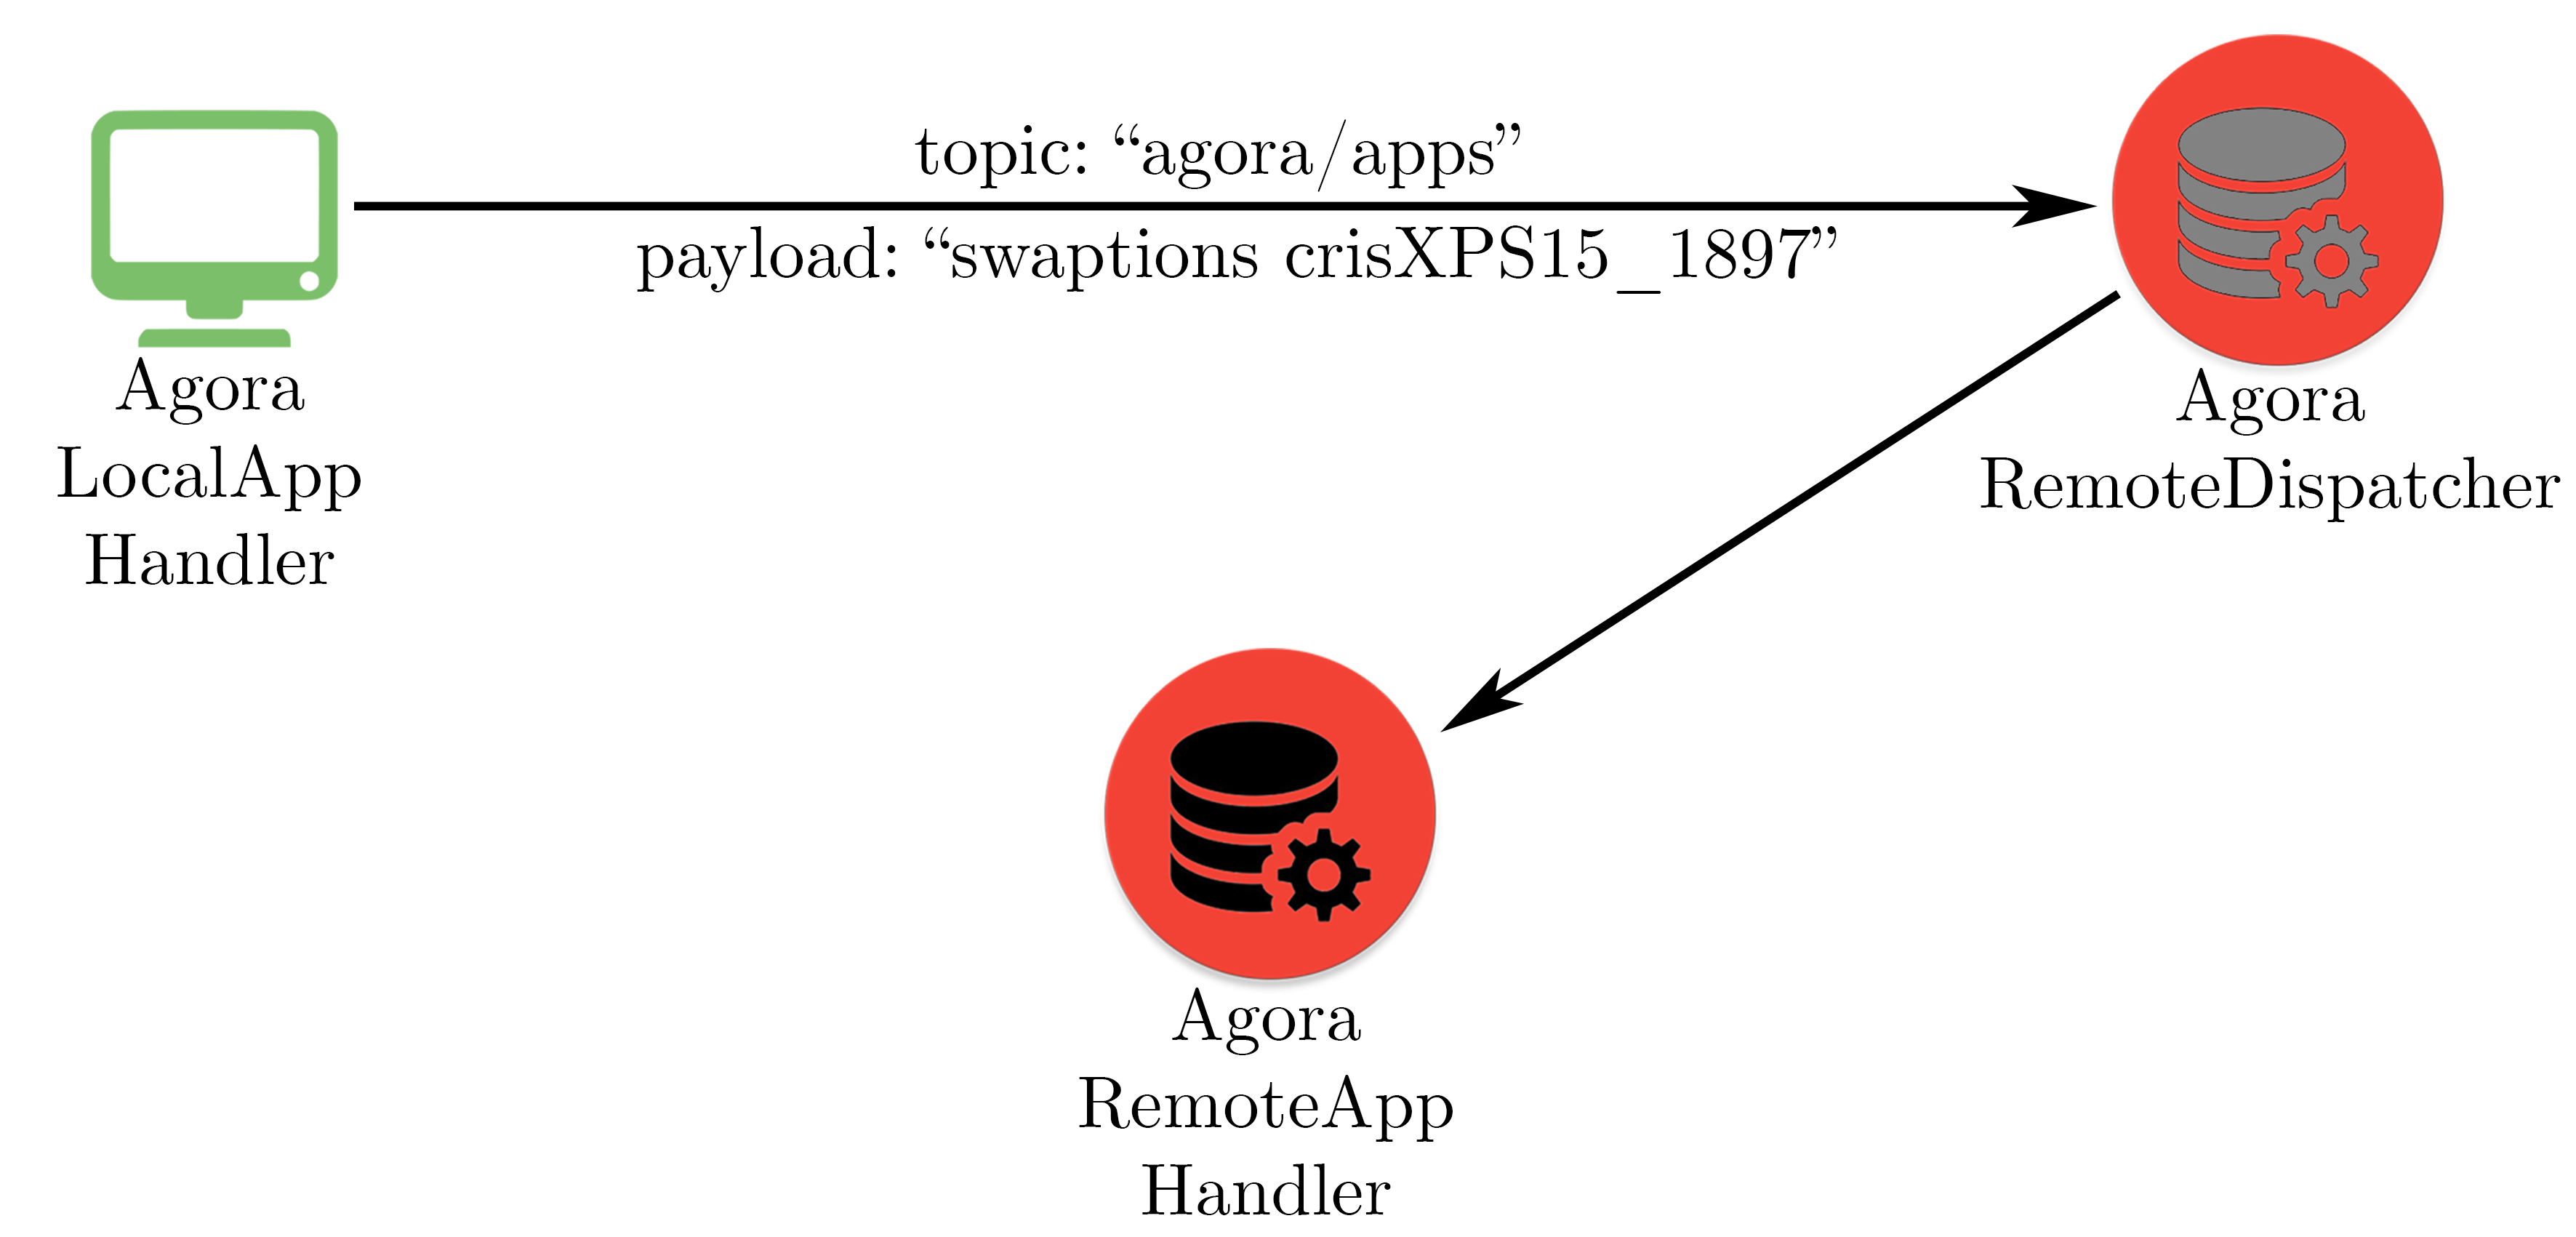
\includegraphics[width = \textwidth]{new_unknown}
    \caption{New unknown application arrival example; a dedicated AgoràRemoteAppHandler module is created by AgoràRemoteDispatcher}
    
\end{figure}

At the beginning, the AgoràLocalAppHandler module subscribes to some topics that are needed to receive communications from the related AgoràRemoteAppHandler:

\begin{enumerate}

    \item "agora/\textit{[appName]}", in order to understand if AgoràRemoteAppHandler has asked application information and, therefore, to reply (see \ref{req_info}); this topic is also used to understand if Agorà\-Remote\-App\-Handler has crashed and, so, to react properly (see \ref{handler_disc});
    
    \item "agora/\textit{[appName]}/\textit{[hostname]\_[PID]}/conf", in order to receive configurations from AgoràRemoteAppHandler during DSE phase (see \ref{dse_conf});
    
    \item "agora/\textit{[appName]}/\textit{[hostname]\_[PID]}/model", in order to receive\linebreak a partial OP list (see \ref{DoEModelSend}) and the complete predicted model from AgoràRemoteAppHandler (see \ref{modelSend}).

\end{enumerate}

\begin{figure}[H]

    \centering
    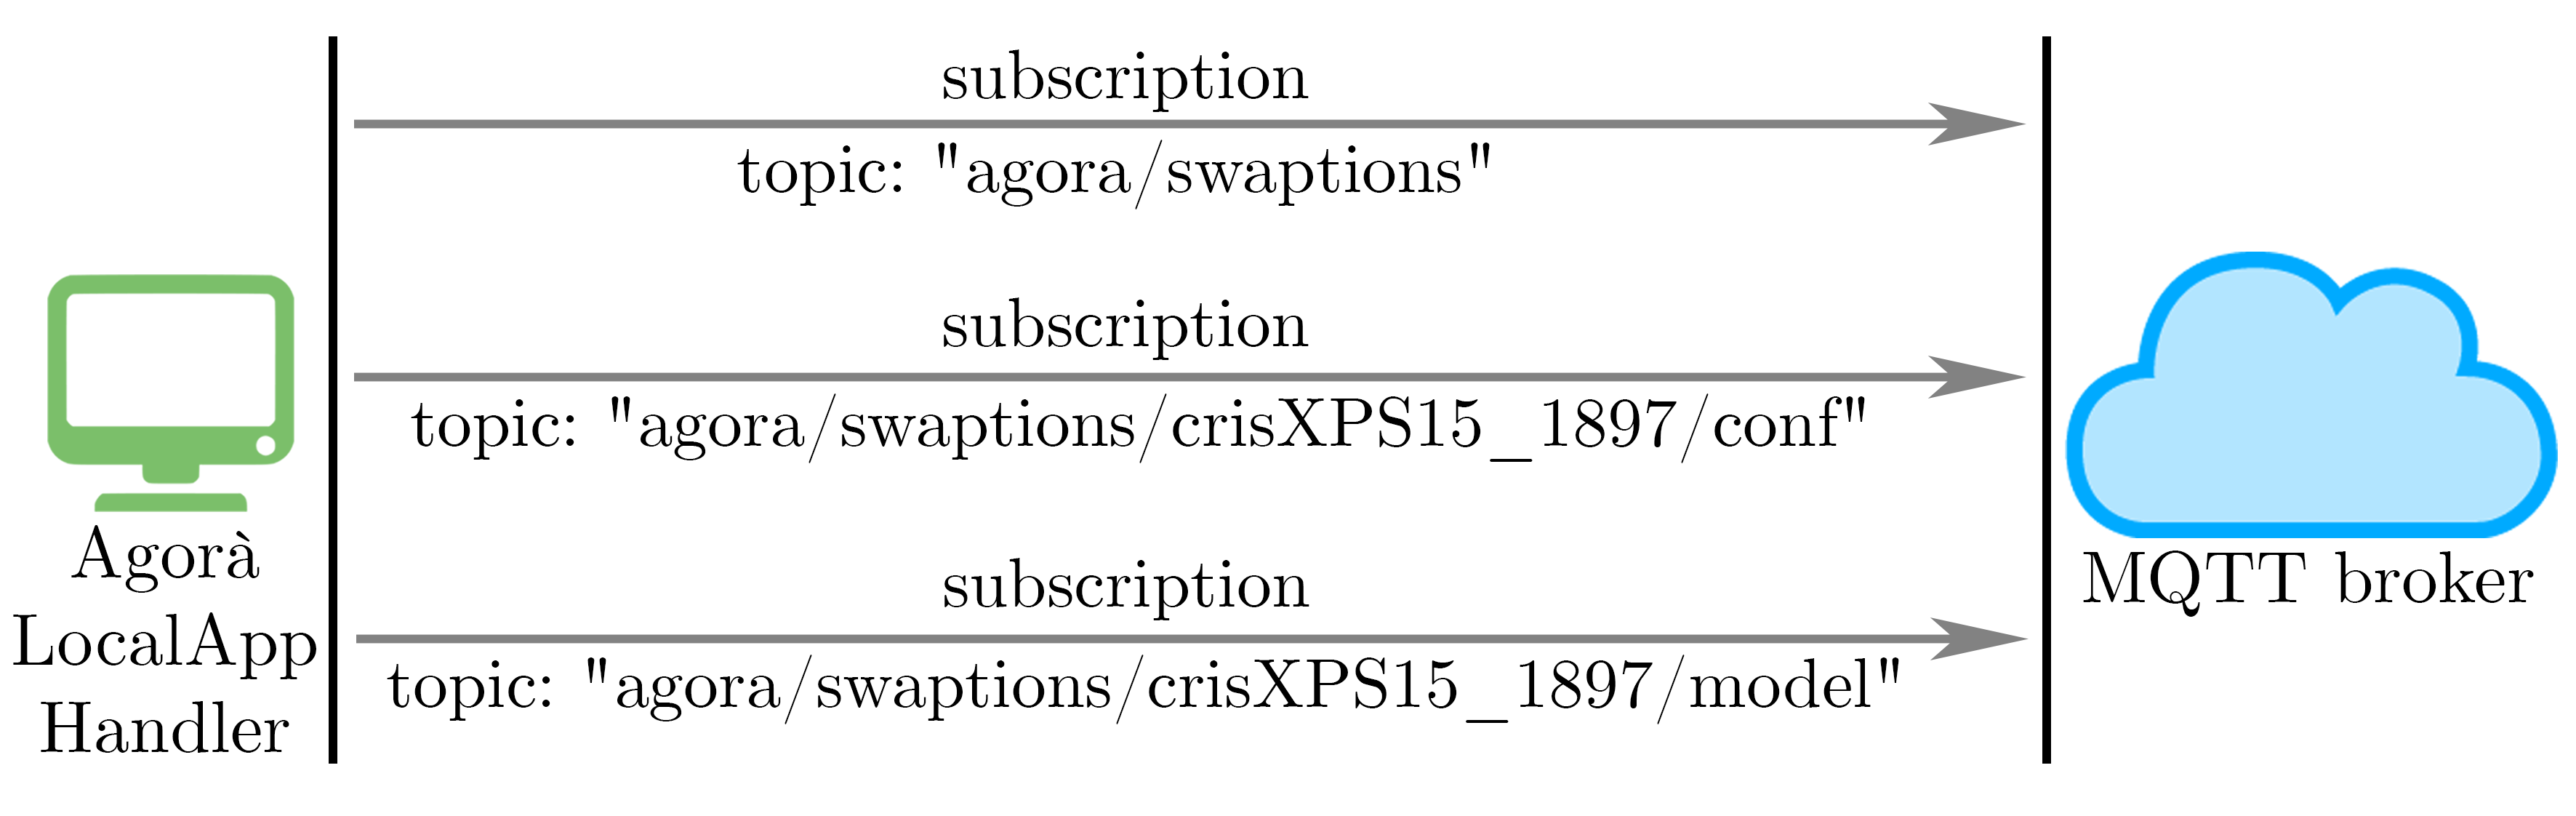
\includegraphics[width = \textwidth]{client_subs}
    \caption{AgoràLocalAppHandler MQTT subscriptions example}
    
\end{figure}

The AgoràRemoteAppHandler module subscribes to some topics in order to manage correctly all various situations that happens:

\begin{enumerate}

    \item "agora/\textit{[appName]}/newHostpid", in order to manage the hypothetical notification of other AgoràLocalAppHandler modules that are supervising the same application (see \ref{knownApp});
    
    \item "agora/\textit{[appName]}/req", in order to manage all the requests made by AgoràLocalAppHandler modules during program execution (see \ref{clientReq});
    
    \item "agora/\textit{[appName]}/info/\#", in order to receive all available application information, such as parameter name and values (see \ref{client_info}); real topic is "agora\slash{}\textit{[appName]}\slash{}info\slash{}\textit{[host\-name]\_ [PID]}" (see MQTT multi-level wildcard, \ref{mqtt}), therefore AgoràRemote\-App\-Handler can store the ID of the node that is sending application information, in order to react properly to node possible crash during this phase (see \ref{client_disc});
    
    \item "agora/\textit{[appName]}/disconnection", in order to correctly react to a possible node disconnection (see \ref{client_disc});
    
    \item "agora/\textit{[appName]}/OPs", in order to receive Operating Points from AgoràLocalAppHandler modules during Design Space Exploration phase (see \ref{opSend}).

\end{enumerate}

\begin{figure}[H]

    \centering
    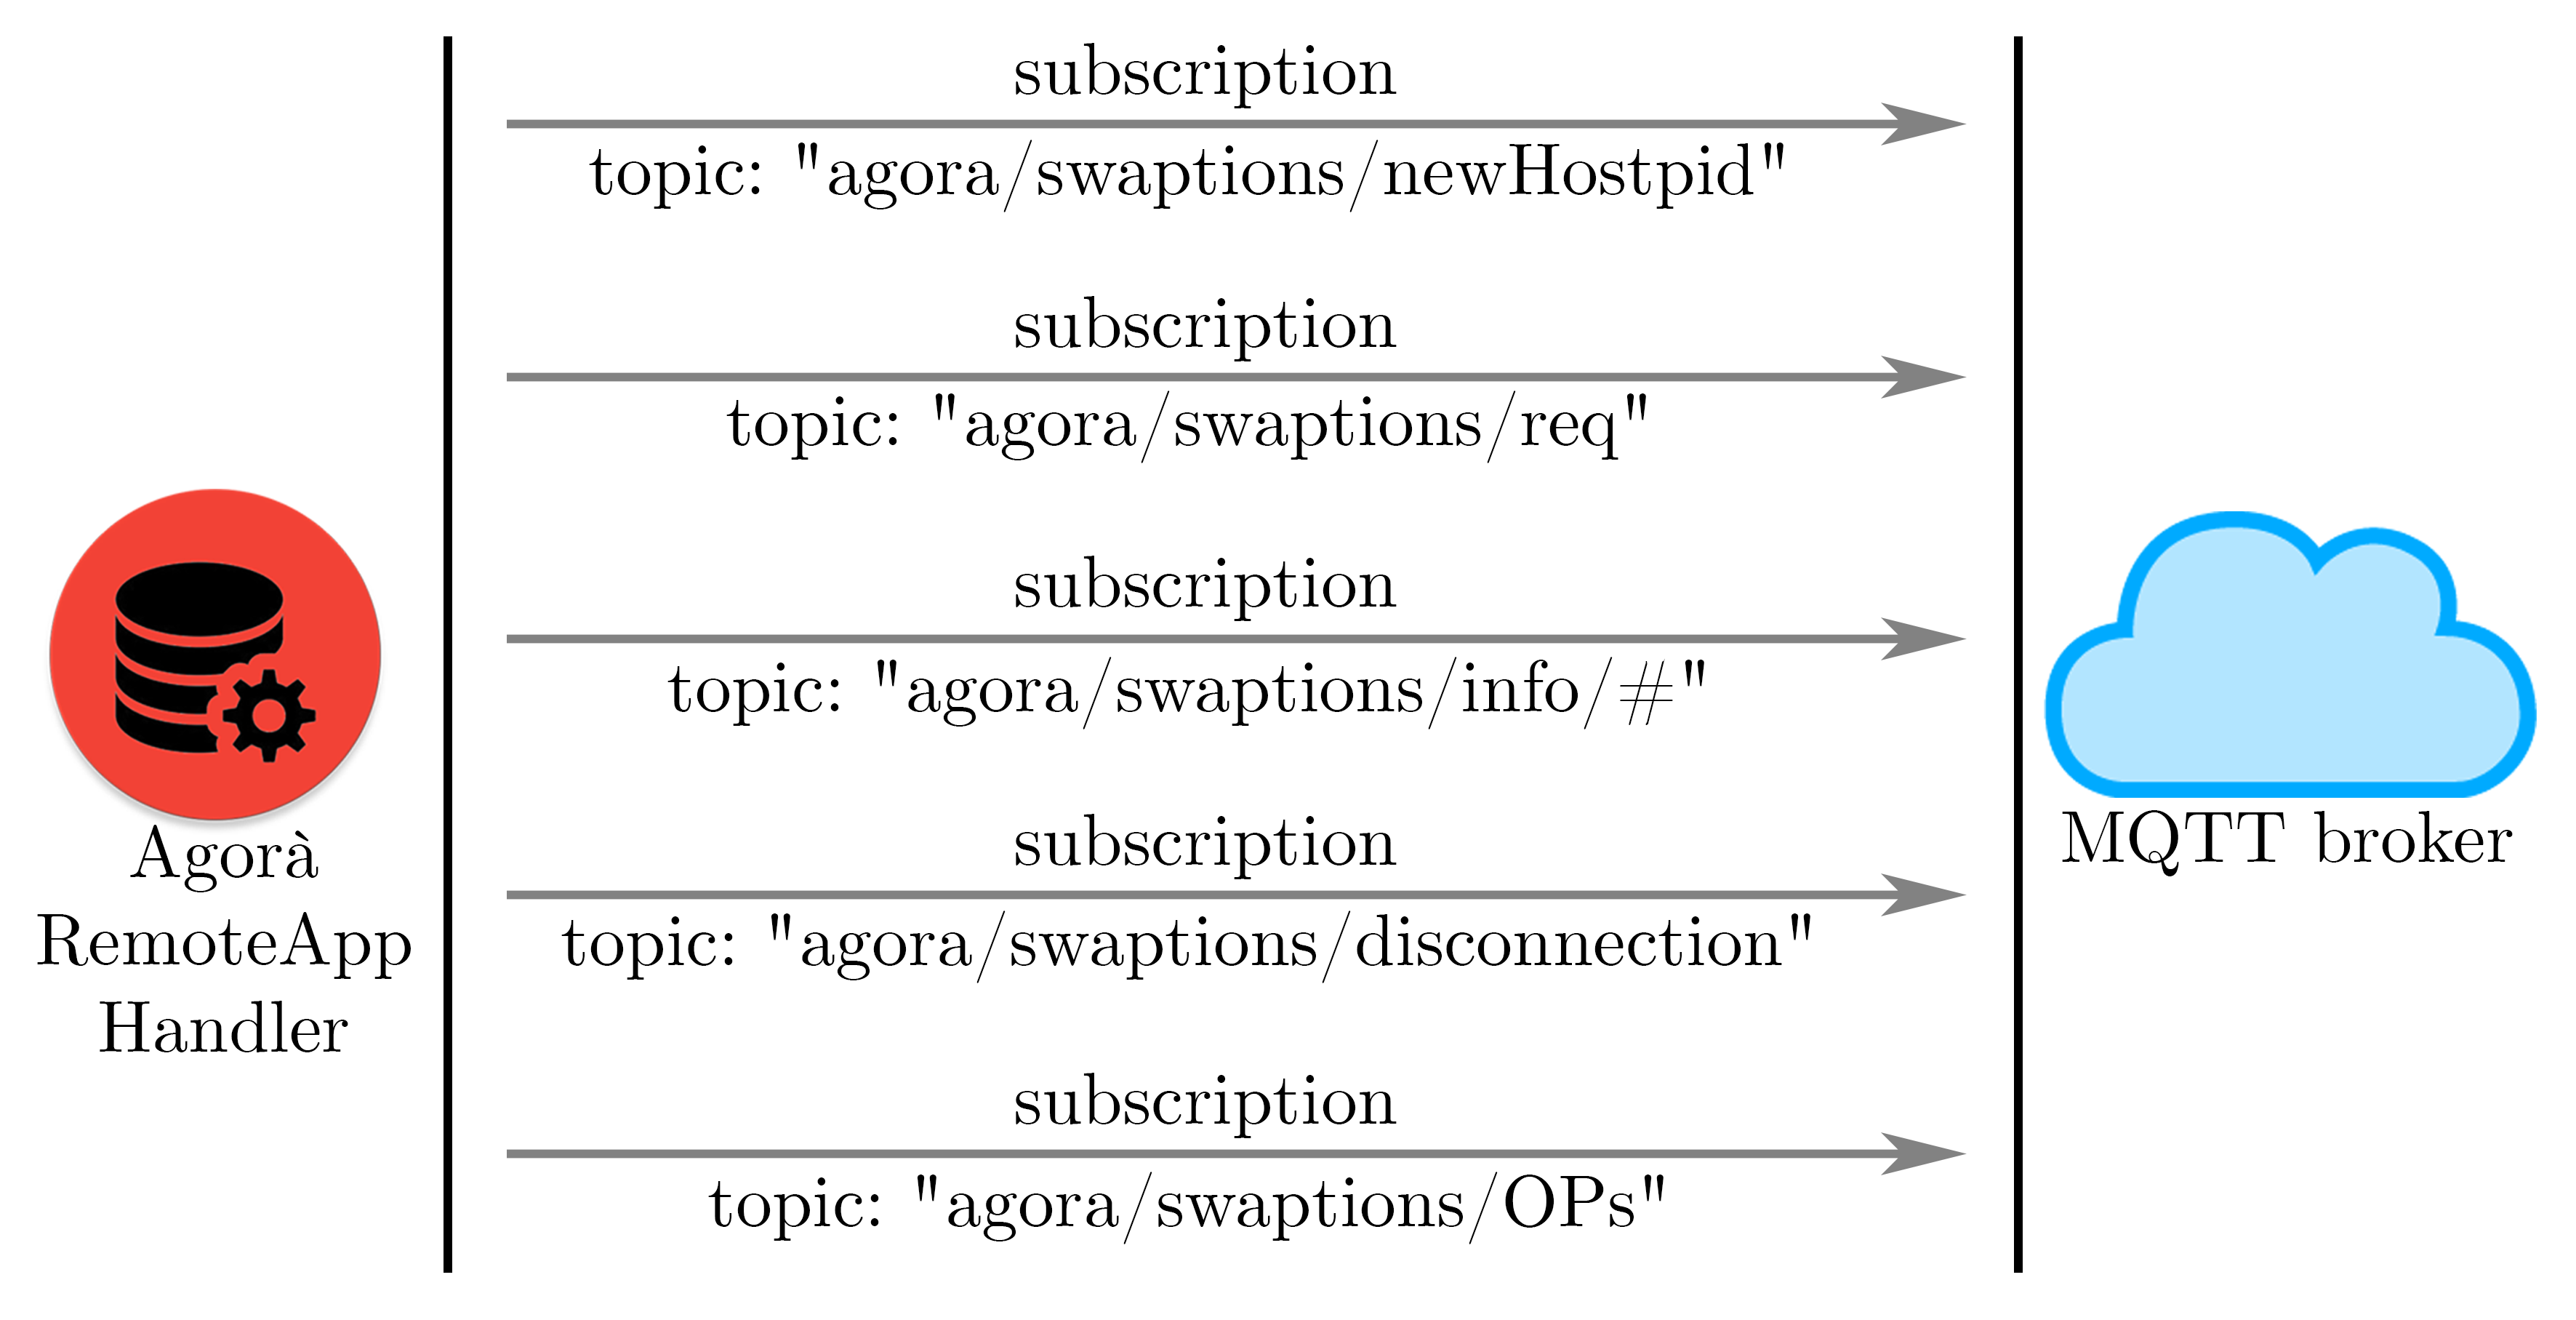
\includegraphics[width = \textwidth]{handler_subs}
    \caption{AgoràRemoteAppHandler MQTT subscriptions example}
    
\end{figure}


\subsubsection{Known application}\label{knownApp}

When the AgoràRemoteDispatcher module is informed that a new node has started running an application but there exist already an AgoràRemoteAppHandler that is managing that program, it publishes on topic "agora/\textit{[appName]}/newHostpid" the new machine hostname plus PID, so that the corresponding AgoràRemoteAppHandler module can add the node to the pool of machines that are running the application it is supervising:

\begin{figure}[H]

    \centering
    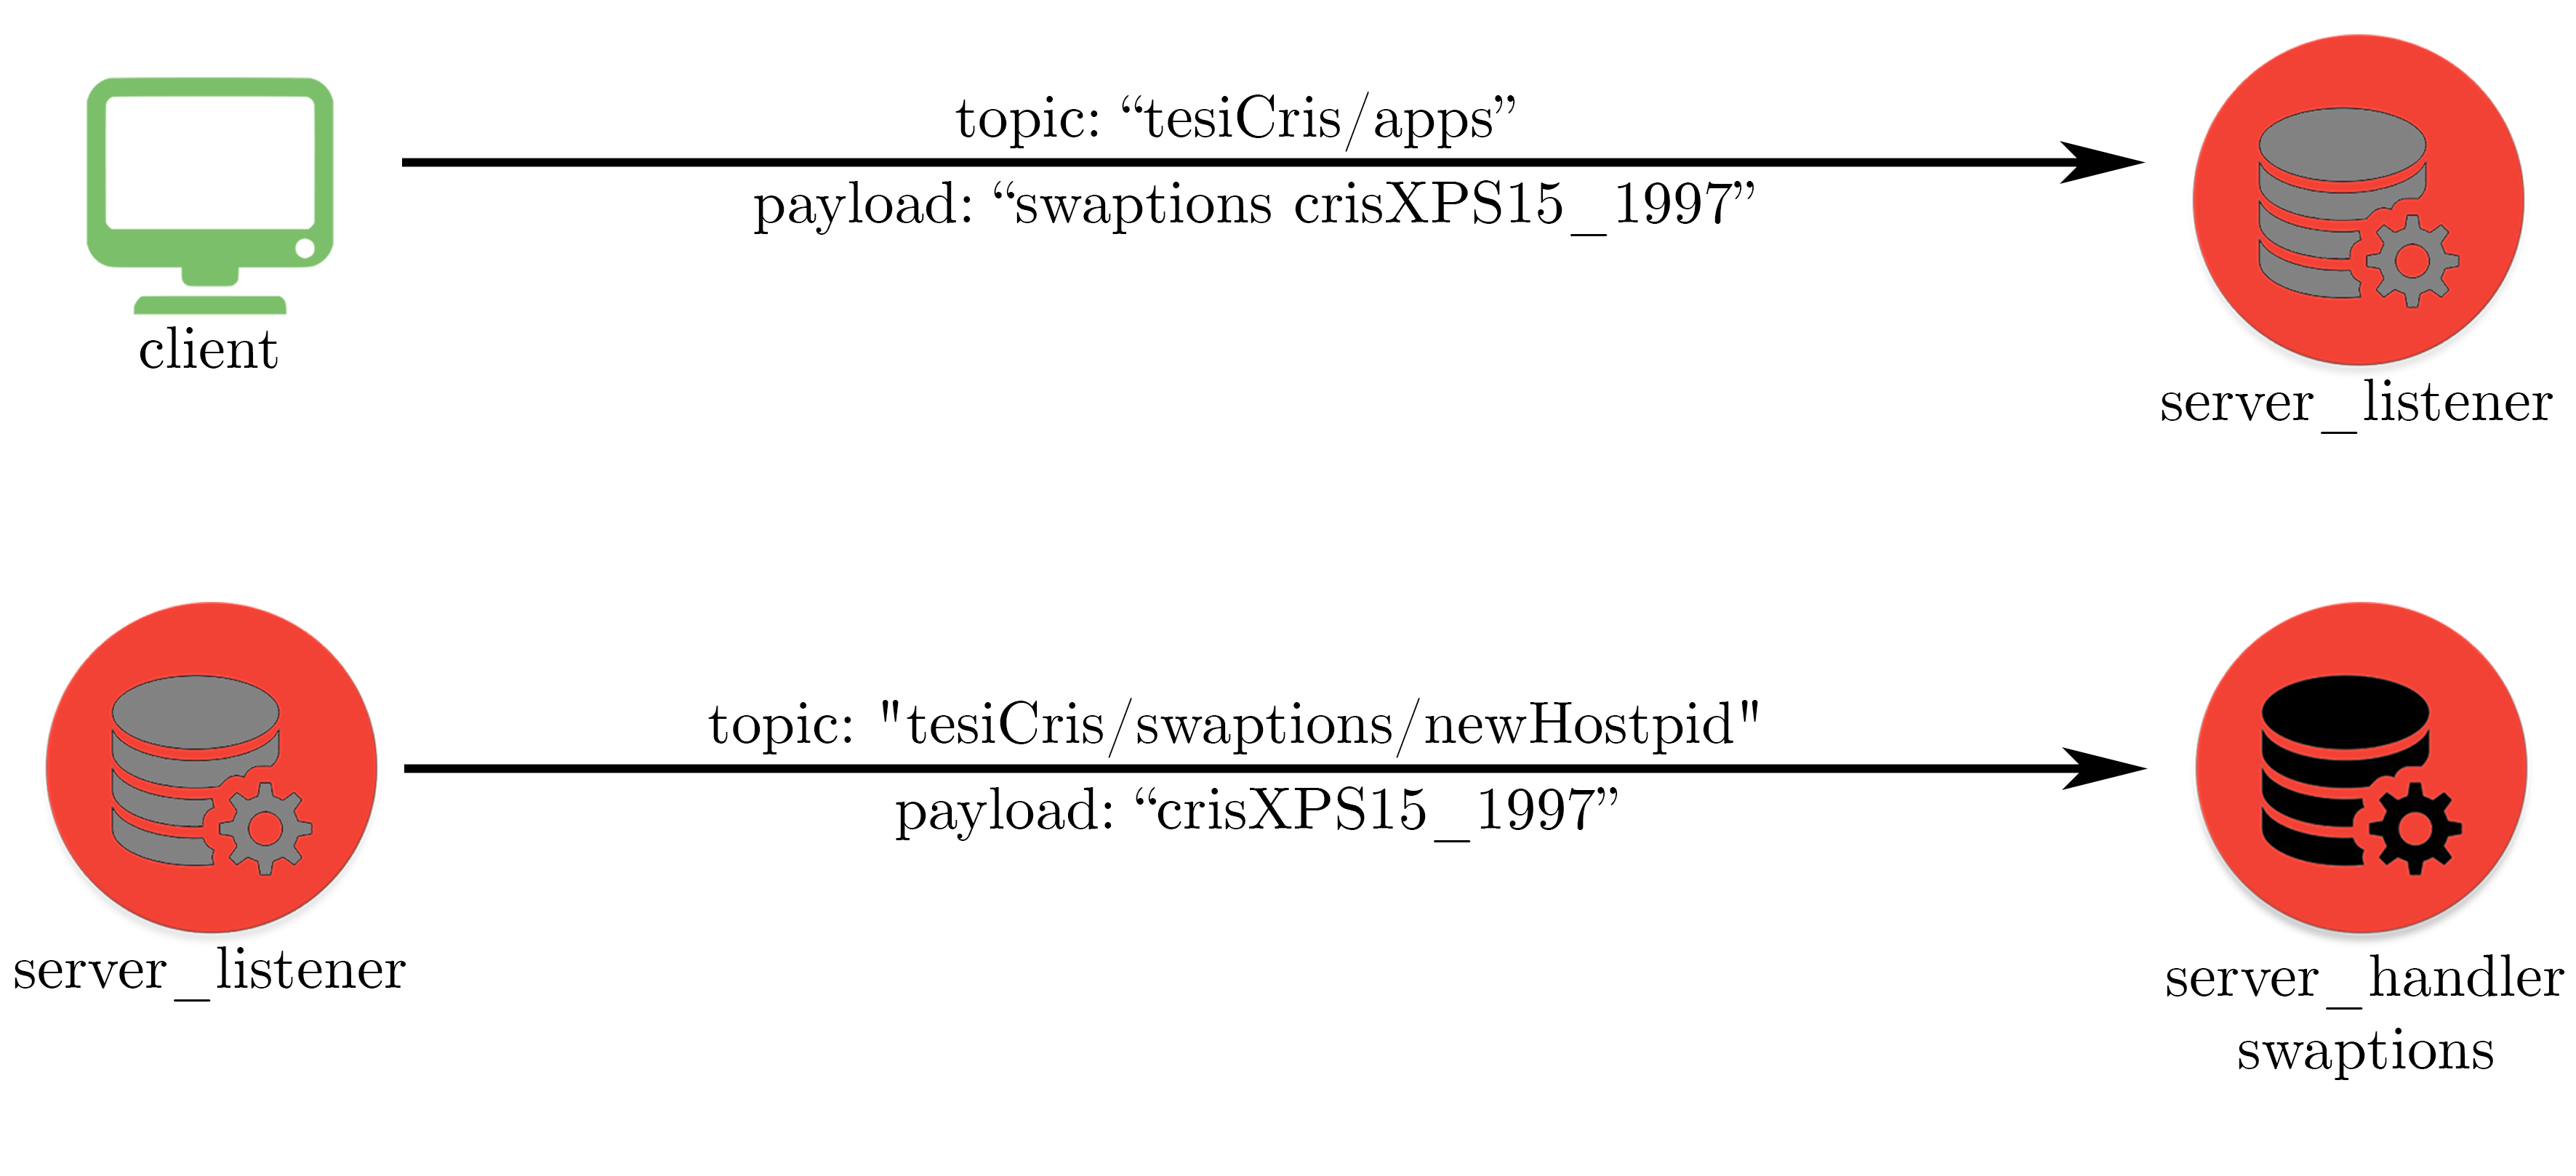
\includegraphics[width = \textwidth]{new_known}
    \caption{New known application arrival example; node ID is sent by AgoràRemoteDispatcher to the corresponding AgoràRemoteAppHandler module}
    
\end{figure}





\subsection{AgoràLocalAppHandler request}\label{clientReq}

At each predetermined time interval, AgoràLocalAppHandler modules make a request to the related AgoràRemoteAppHandler, publishing their hostname plus PID on topic "agora/\textit{[appName]}/req":

\begin{figure}[H]

    \centering
    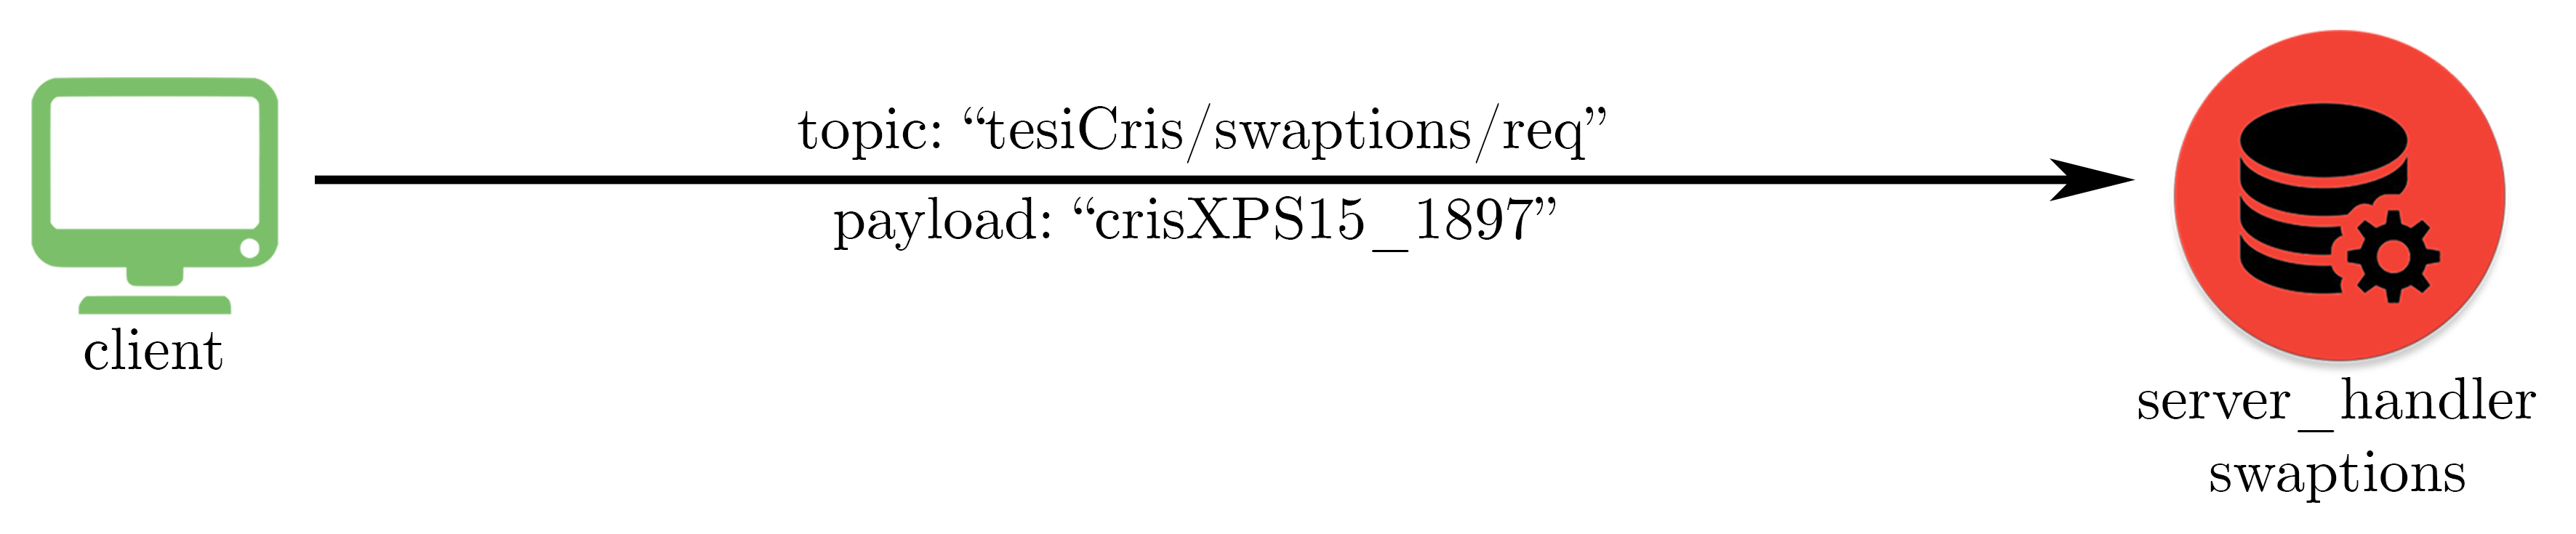
\includegraphics[width = \textwidth]{req}
    \caption{AgoràLocalAppHandler request example}
    
\end{figure}

This kind of publication is repeated until the node receives the predicted complete Operating Point list; AgoràRemoteAppHandler replies to these requests according to its internal state, that can be one of the following:

\begin{enumerate}

    \item \textit{unknown};

    \item \textit{receivingInfo};

    \item \textit{buildingDoE};

    \item \textit{DSE};

    \item \textit{buildingTheModel};

    \item \textit{autotuning}.

\end{enumerate}


\subsubsection{AgoràRemoteAppHandler internal state equal to \textit{unknown}}\label{req_info}

AgoràRemoteAppHandler doesn't know anything about the application it is managing, except its name; it asks to AgoràLocalAppHandler modules all available information, making a publication with payload "info" on topic "agora/\textit{[appName]}":

\begin{figure}[H]

    \centering
    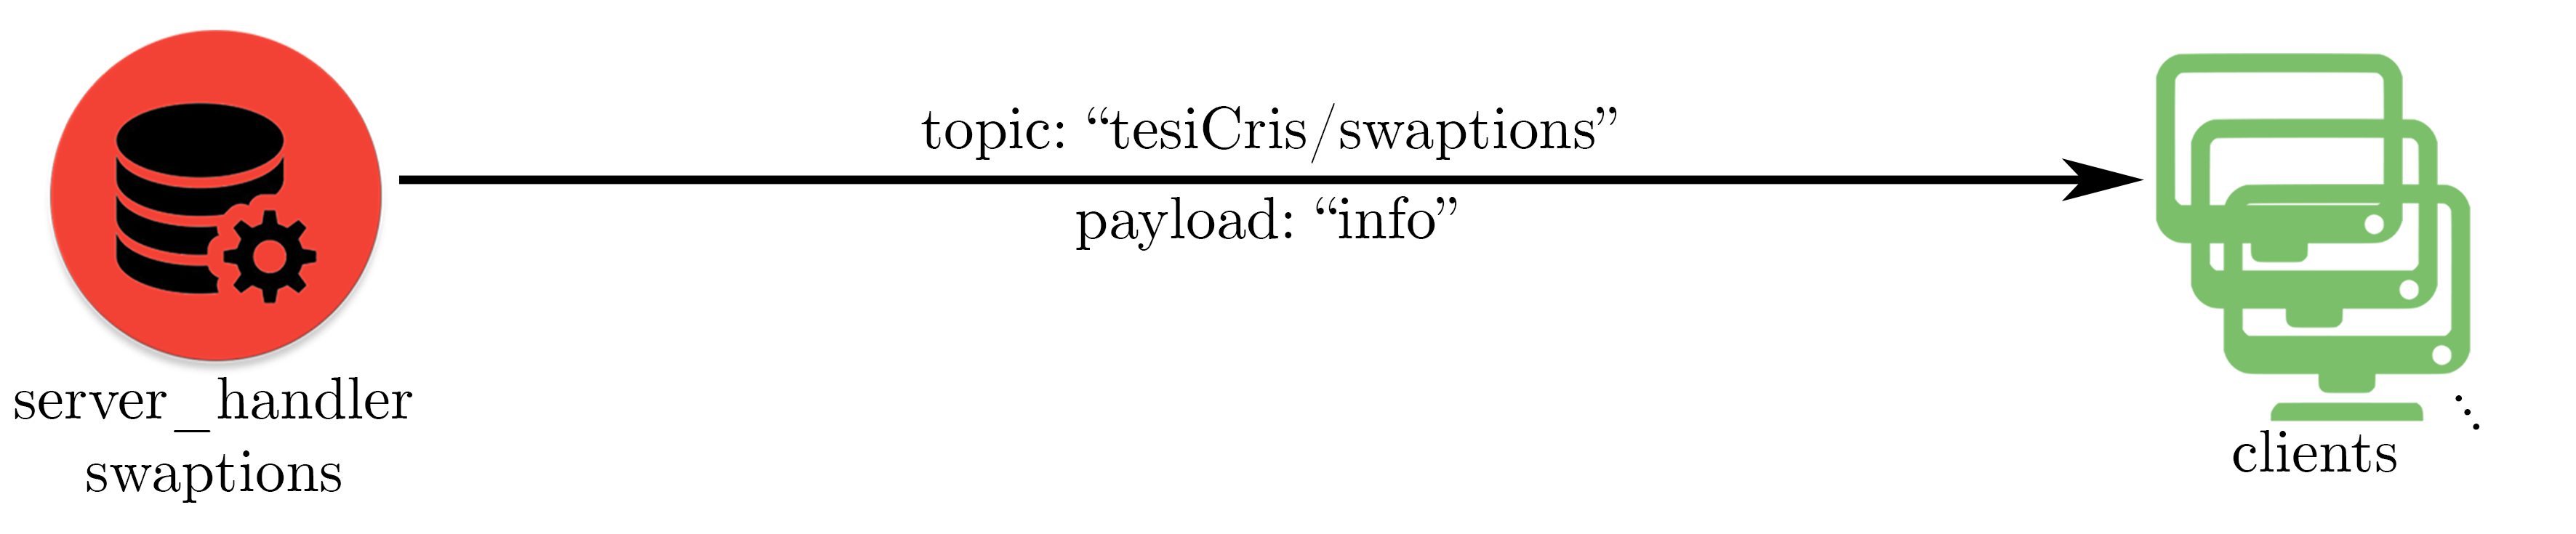
\includegraphics[width = \textwidth]{info_req}
    \caption{Application information request by \textit{AgoràRemoteAppHandler} example}
    
\end{figure}


\subsubsection{AgoràRemoteAppHandler internal state equal to \textit{receivingInfo}}

The AgoràRemoteAppHandler module is receiving application information, so in this case it discards all possible requests made by AgoràLocalAppHandler modules.


\subsubsection{AgoràRemoteAppHandler internal state equal to \textit{buildingDoE}}

AgoràRemoteAppHandler, according to the received Design of Experiments type (see \ref{client_info}), is building the set of configurations that are going to be distributed to AgoràLocalAppHandler modules during Design Space Exploration phase; also in this case it discards all possible AgoràLocalAppHandler module requests.


\subsubsection{AgoràRemoteAppHandler internal state equal to \textit{DSE}}\label{dse_conf}

The AgoràRemoteAppHandler module has computed DoE configurations, so it is driving Design Space Exploration phase; it picks up the first element on top of the available configuration list and it sends, in lexicographic order, the associated software knob values on topic "agora\slash{}\textit{[appName]}\slash{}\textit{[hostname]\_[PID]}\slash{}conf", relative to the AgoràLocalAppHandler module that made the request; the configuration just sent is reinserted at the end of the mentioned list:

\begin{figure}[H]

    \centering
    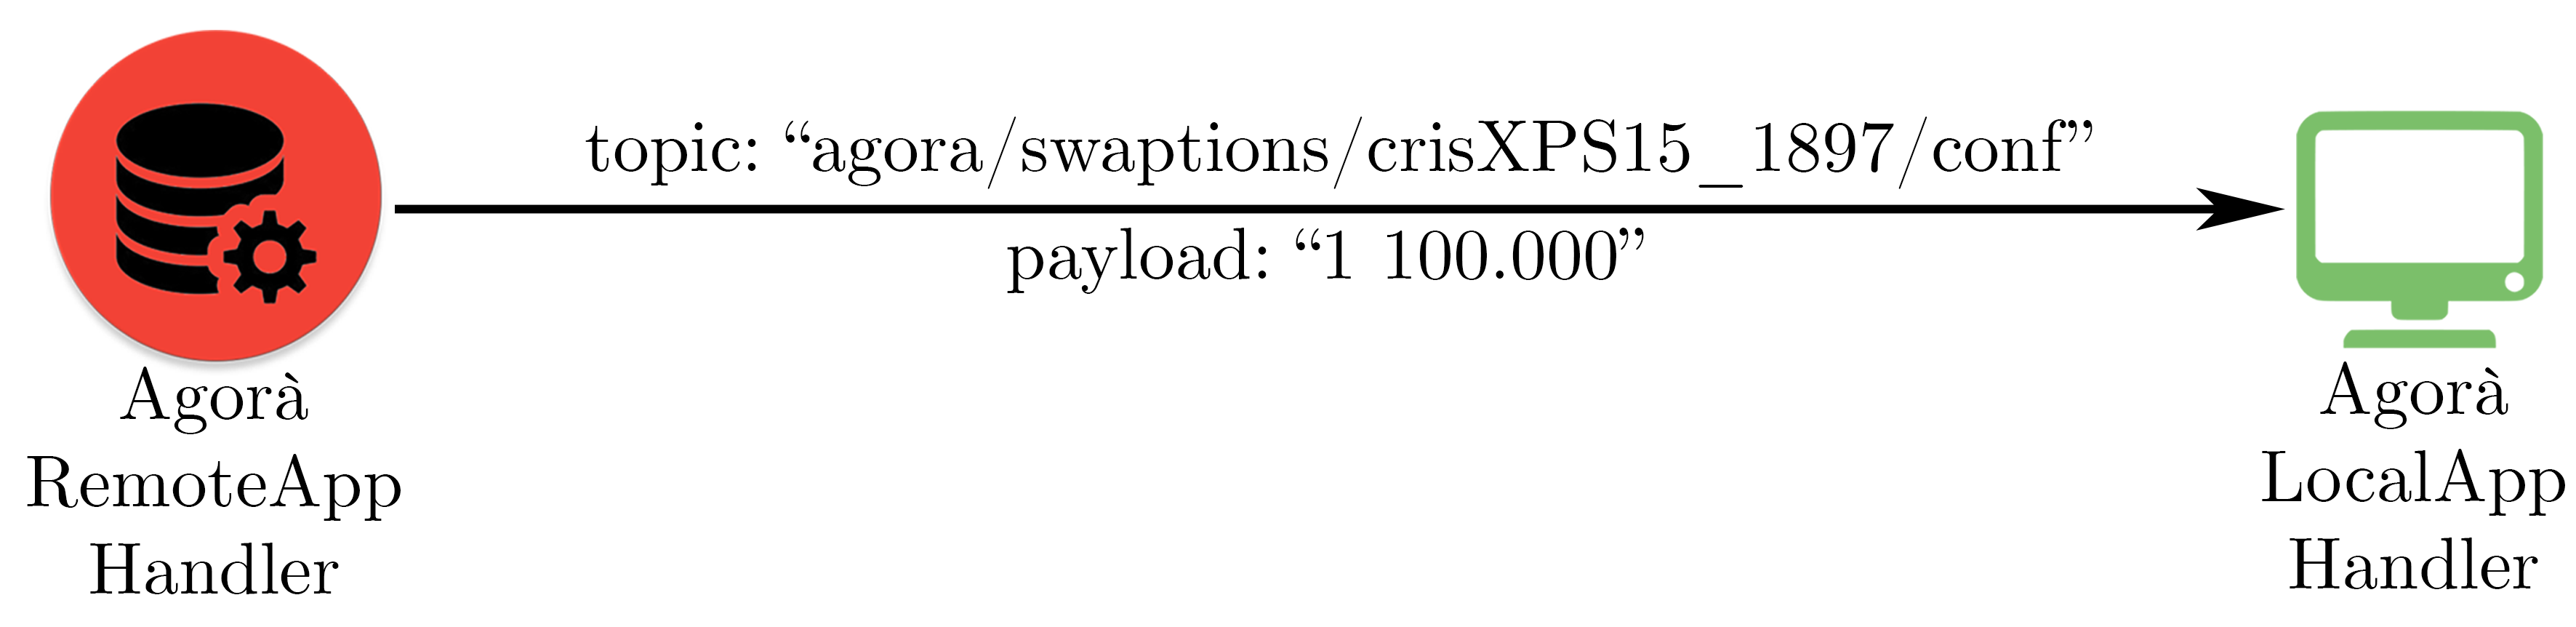
\includegraphics[width = \textwidth]{conf}
    \caption{Configuration dispatch by \textit{AgoràRemoteAppHandler} example}
    \label{fig:conf}
    
\end{figure}

As shown in figure \ref{fig:conf}, AgoràLocalAppHandler receives a configuration with $num\_threads = 1$ and $num\_trials = 100.000$; next computation is going to be done with these parameter values.


\subsubsection{AgoràRemoteAppHandler internal state equal to \textit{building\-The\-Model}}\label{DoEModelSend}

AgoràRemoteAppHandler has gathered all needed OPs related to DoE configurations and it is computing complete Operating Point list through Machine Learning techniques; from gathered Operating Points, a partial model is built, assembling to every DoE configuration the mean of metric values, taken from the corresponding Operating Points; this partial model in sent to the AgoràLocalAppHandler module that made the request: each obtained OP is published on topic "agora/\textit{[appName]}/\textit{[hostname]\_[PID]}/model" with format "\textit{[configuration] [metric values]}"; both configuration and metric values follow lexicographic order; finally, AgoràRemoteAppHandler makes a final publication on same topic with payload "DoEModelDone":

\begin{figure}[H]

    \centering
    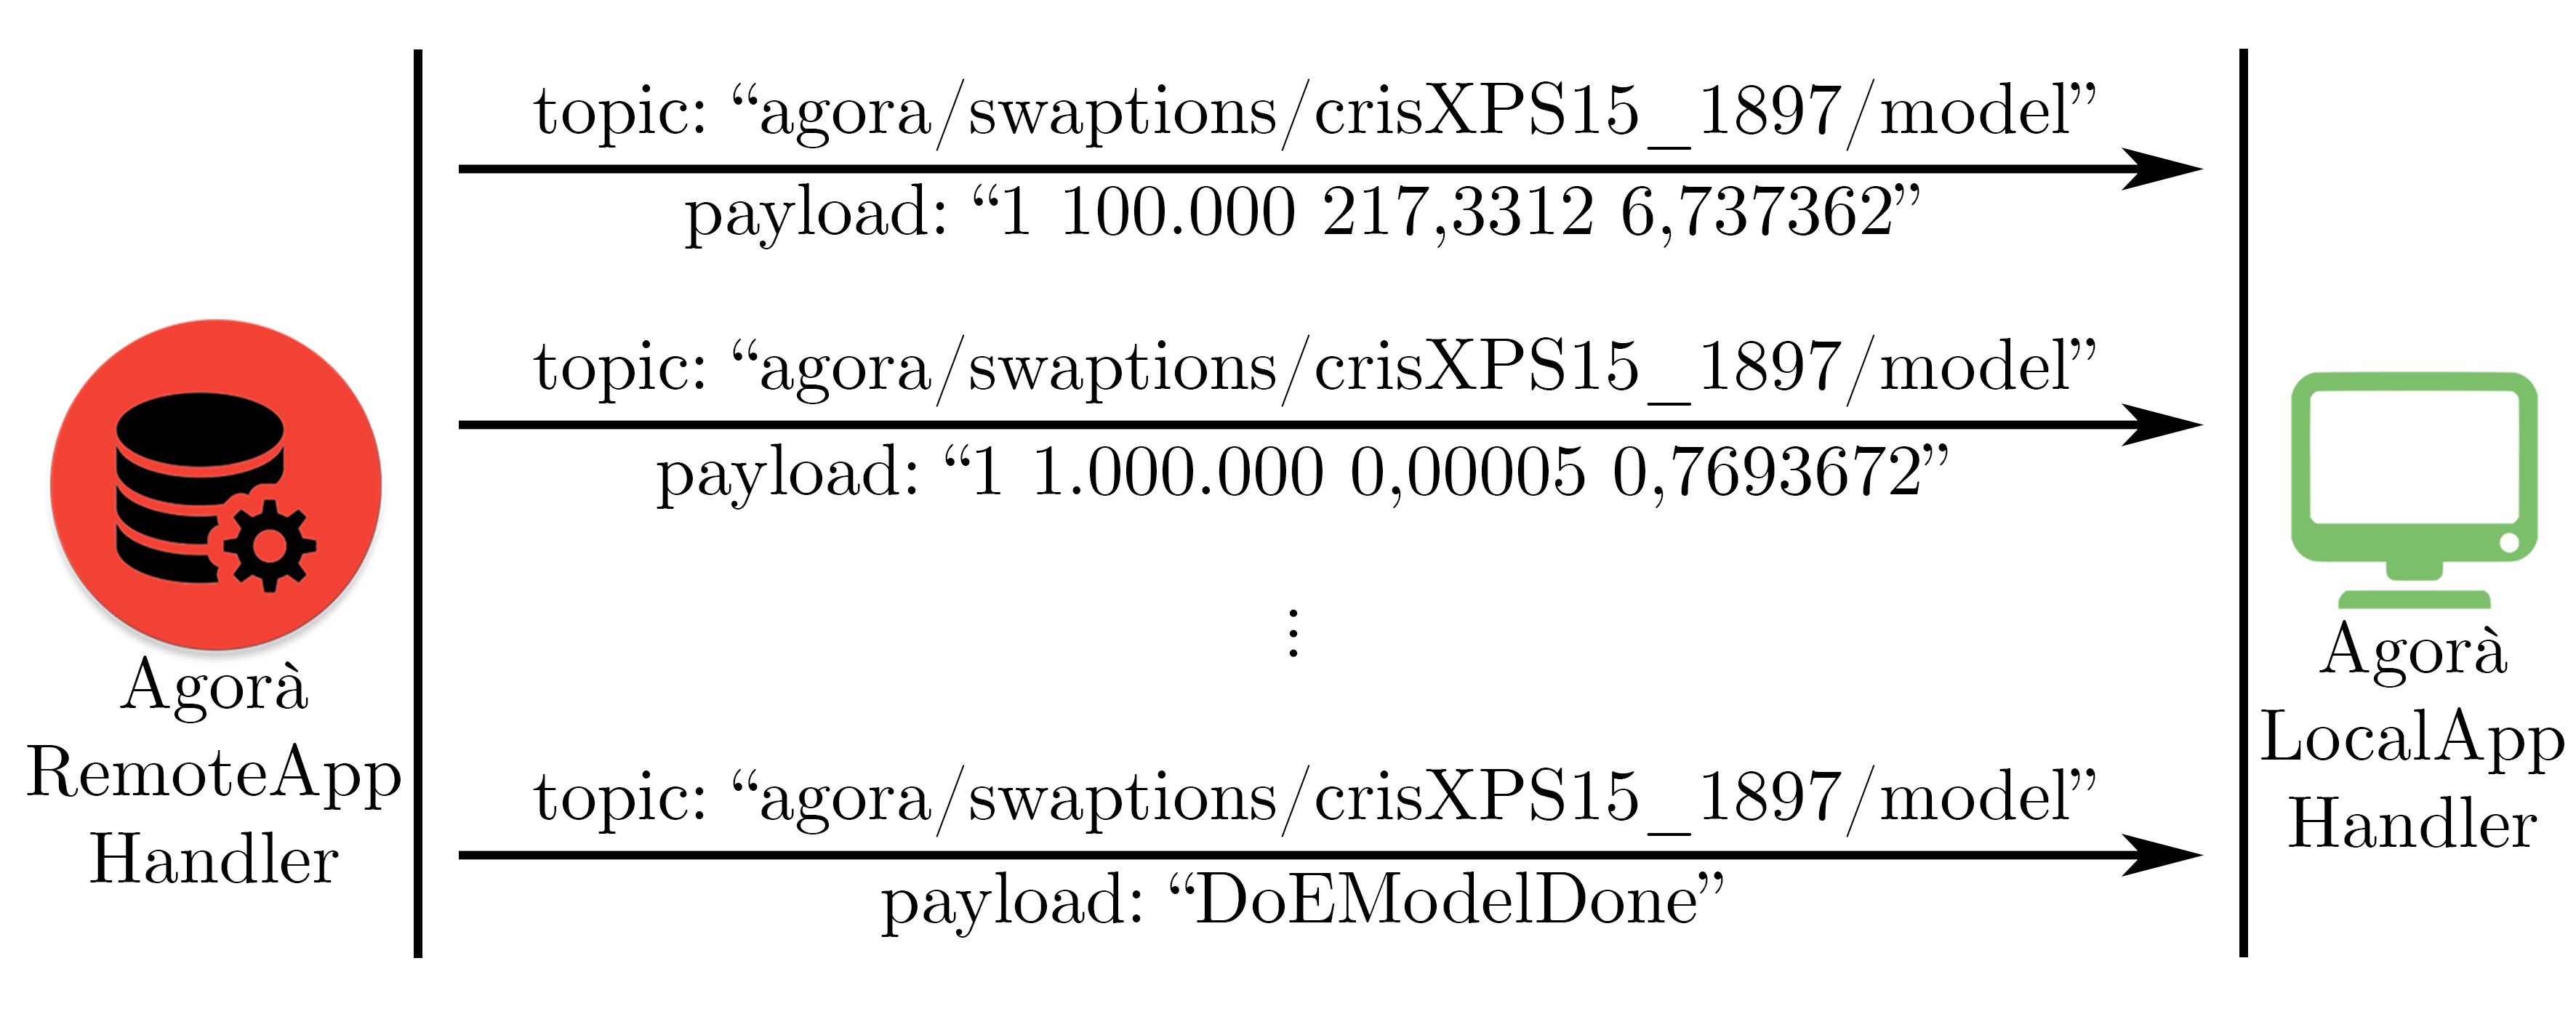
\includegraphics[width = \textwidth]{doe_model}
    \caption{Partial model dispatch by \textit{AgoràRemoteAppHandler} example}
    \label{fig:doe_model}
    
\end{figure}

Taking figure \ref{fig:doe_model} as reference, the first sent OP has parameters\linebreak $num\_threads = 1$ and $num\_trials = 100.000$, with metrics $avg\_error = 217,3312$ and $avg\_throughput = 6,737362$; the AgoràLocalAppHandler module sets up mARGOt autotuner with this OP list, so the application is executed with the best Operating Point that fulfills current goals and requirements.


\subsubsection{AgoràRemoteAppHandler internal state equal to \textit{autotuning}}\label{modelSend}

The AgoràRemoteAppHandler module owns the complete OP list, obtained through the Generalized Linear Regression interface by A\-pach\-e Spark\textsuperscript{TM} MLlib library; similarly to the previous case (\ref{DoEModelSend}), every Operating Point is sent to AgoràLocalAppHandler on topic "agora\slash{}\textit{[app\-Name]}\slash{}\textit{[host\-name]\_[PID]}\slash{}model" with format "\textit{[configuration] [metrics values]}", respecting lexicographic order for both parameter and metric values; the final publication has payload "modelDone":

\begin{figure}[H]

    \centering
    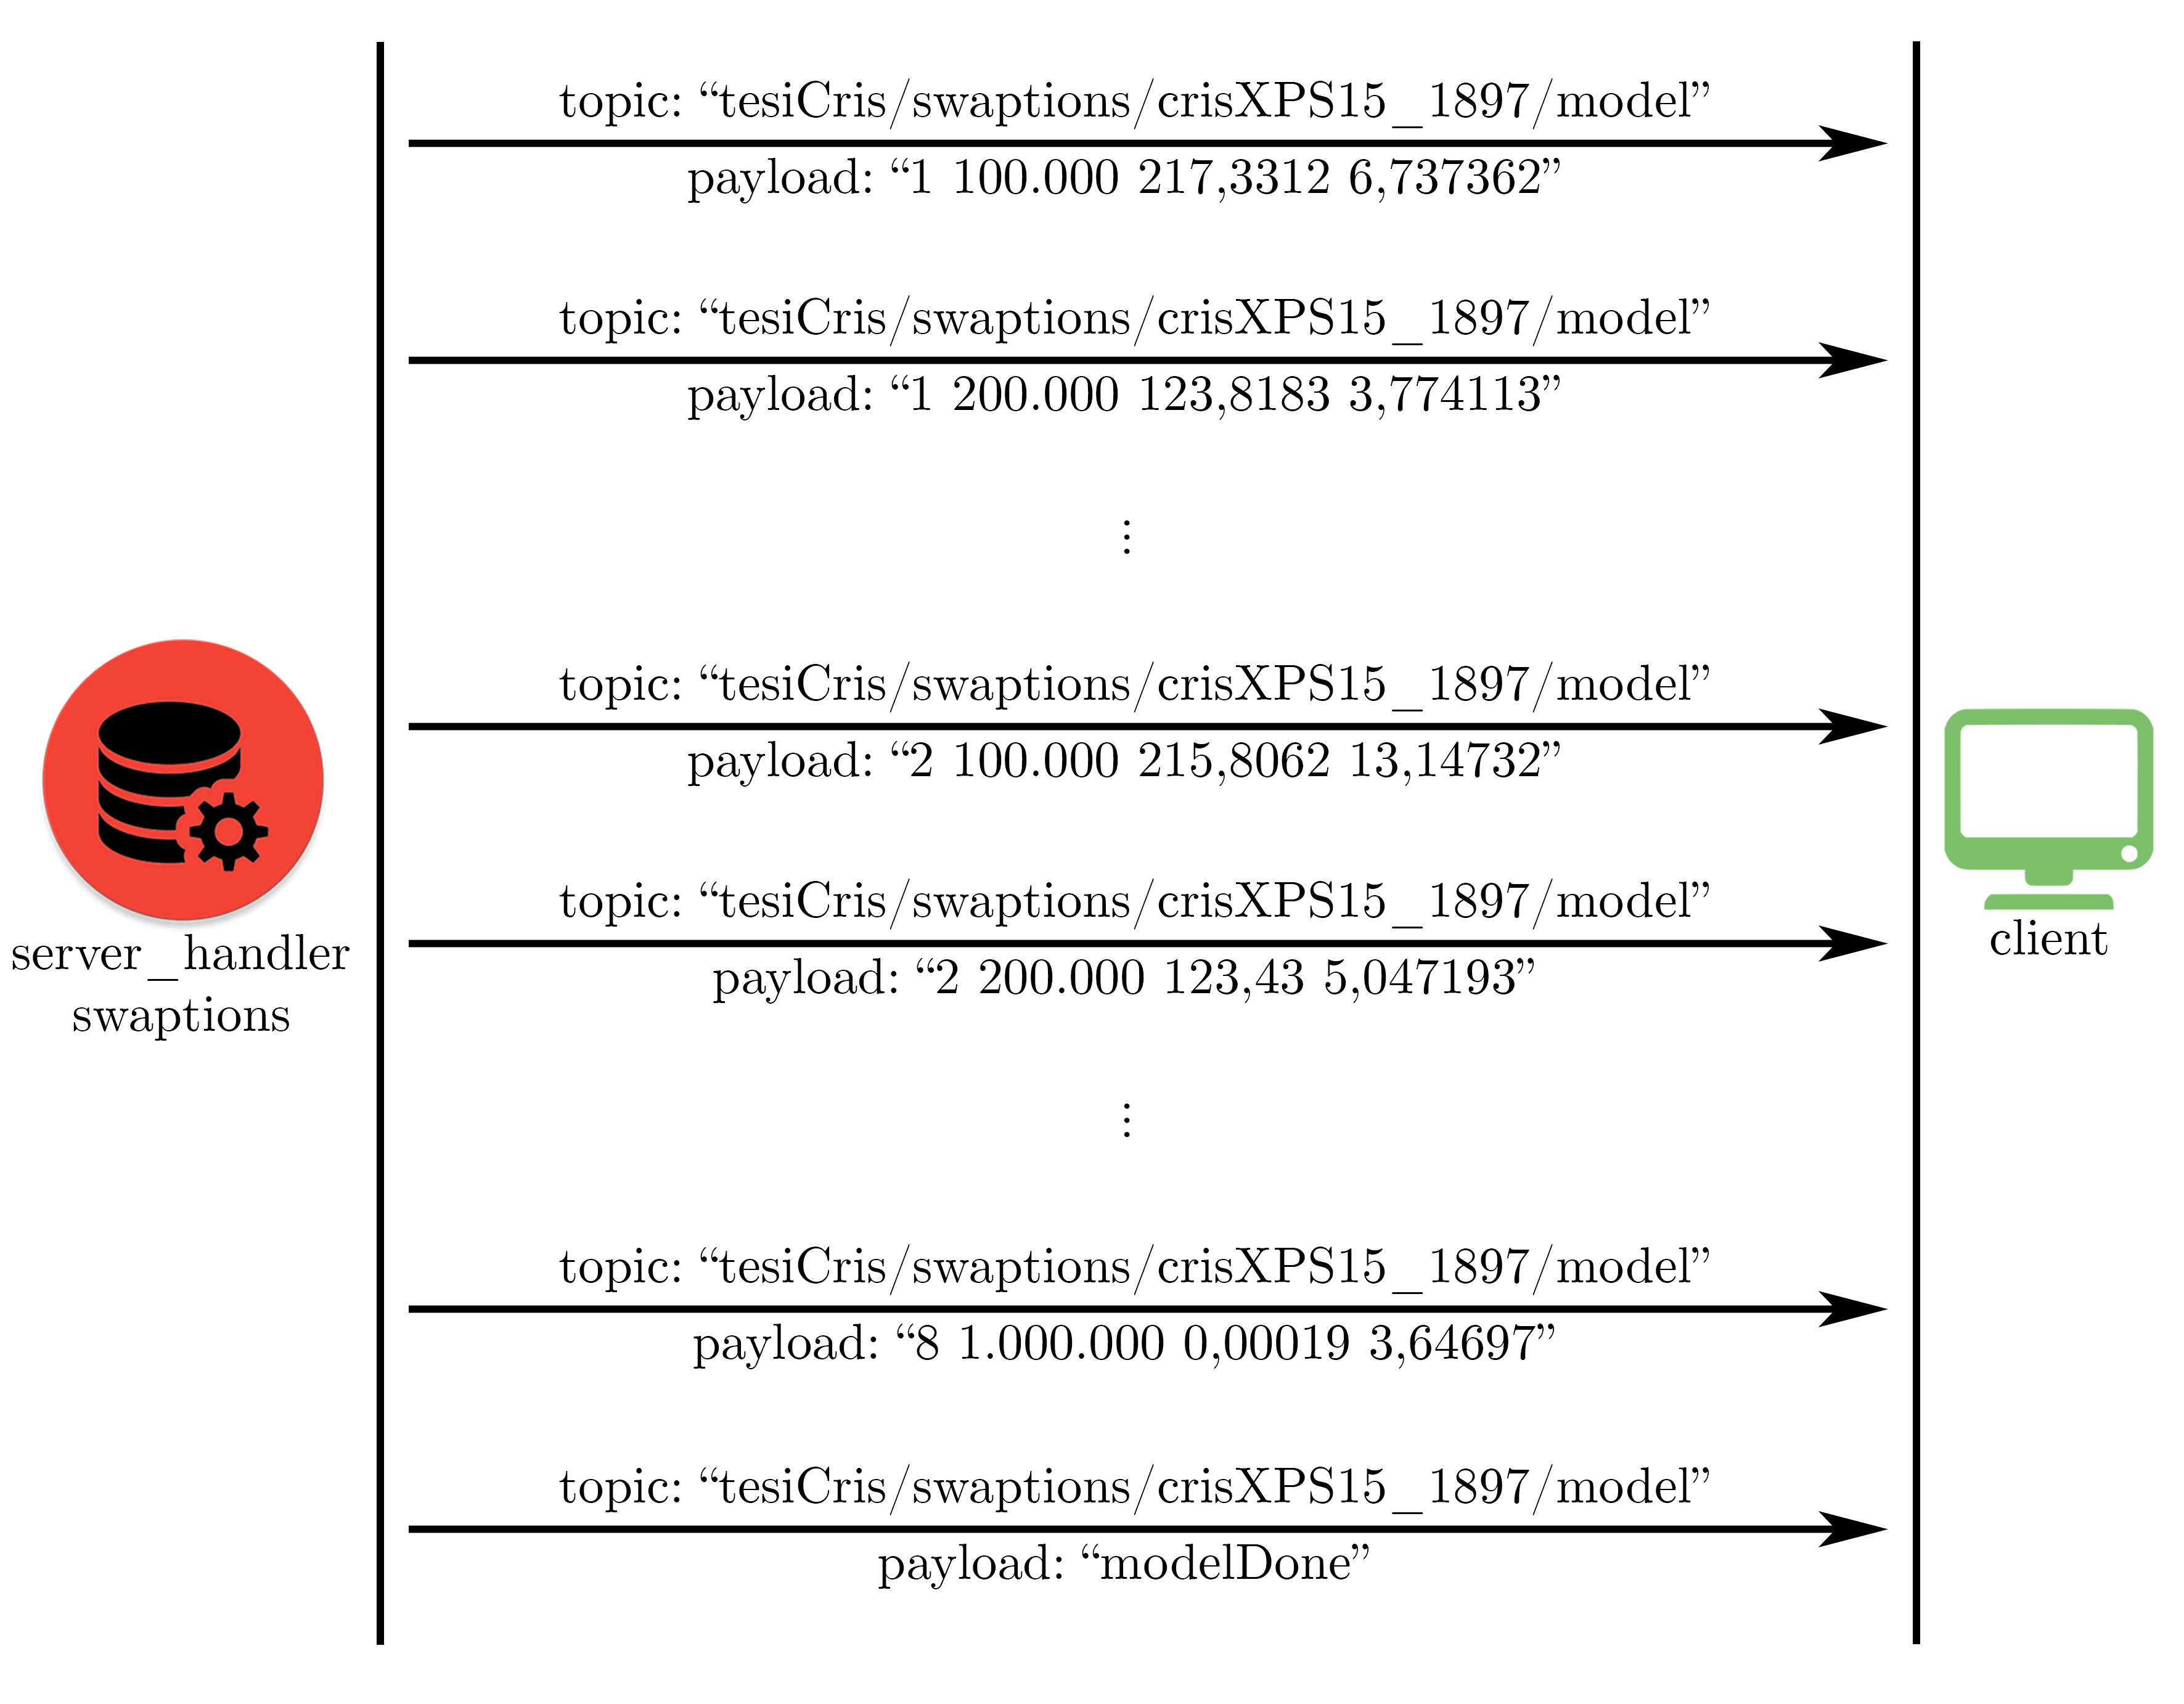
\includegraphics[width = \textwidth]{model}
    \caption{Complete model dispatch by \textit{AgoràRemoteAppHandler} example}
    \label{fig:model}
    
\end{figure}

In Swaptions application, parameter $num\_threads$ can assume 8 different values, while parameter $num\_trials$ 10 ones, so the complete model is composed by all the 80 OPs; after mARGOt autotuner has received all the predicted Operating Points, it can set up application knobs according to current objectives.

From this point on, AgoràLocalAppHandler stops making requests to the AgoràRemoteAppHandler module.





\subsection{Application information dispatch by AgoràLocalAppHandler}\label{client_info}

It has been shown that, if an AgoràRemoteAppHandler module receives a request from a node but its internal state is \textit{unknown}, it requests application information (see \ref{req_info}); AgoràRemoteAppHandler saves both the identifier of the first AgoràLocalAppHandler module that replies and all data it receives; other possible replies from other AgoràLocalAppHandler modules are discarded.

Mandatory information that AgoràLocalAppHandler modules have to send is:

\begin{enumerate}

    \item metrics under examination: the keyword is \textit{metric}, followed by metric name; there is a publication for each metric; publications have to be in lexicographic order with respect to metric name;
    
    e.g. payload: "metric avg\_throughput"
    
    \item application parameters: the keyword is \textit{param}, followed by parameter name, the way in which it is transmitted and corresponding values; there is a publication for each parameter; also in this case, publications must follow lexicographic order with respect to parameter name; Agorà makes available two ways to send values:
    
    \begin{enumerate}
    
        \item by list: the keyword is \textit{enum} and, in this case, all possible values are listed;
        
        \item by extreme values and step: the keyword is \textit{range} and, in this case, minimum value, maximum value and step are sent; AgoràRemoteAppHandler module, from this information, computes all possible parameter values.
    
    \end{enumerate}
    
    e.g. payload: "param num\_threads enum 1 2 3 4 5 6 7 8"
    
    e.g. payload: "param num\_trials range 100.000 1.000.000 100.000"

\end{enumerate}

There are some optional information that AgoràLocalAppHandler modules can send to the AgoràRemoteAppHandler:

\begin{enumerate}

    \item number of required repetitions for each Operating Point: the keyword is \textit{numReps}, followed by a number; this value represents the number of Operating Points that the AgoràRemoteAppHandler has to gather for each Design of Experiments configuration, during Design Space Exploration phase;
    
    e.g. payload: "numReps 5"
    
    \item Design of Experiments type: the keyword is \textit{DoE}, followed by the term that indicates the kind of Design of Experiments that has to be used; it can be:
    
    \begin{enumerate}
    
        \item \textit{fcccd}: it corresponds to the Face Centered Central Composite DoE with one Center Point;
        
        \item \textit{ff2l}: it corresponds to the 2-Level Full-Factorial DoE;
        
        \item \textit{pbd}: it corresponds to the Plackett-Burman DoE;
        
        \item \textit{lhd}: it corresponds to the Latin-Hypercube DoE; in this case, there is another optional information that can be sent to the AgoràRemoteAppHandler module: the number of configurations that have to be produced, with the word \textit{lhdSamples} followed by the desired value; if this information is not sent, the number of random configurations is equal to the number of application parameters;
        
        \item \textit{fcccdExtra}: it corresponds to the Face Centered Central Composite DoE with one Center Point plus the addition of other configurations through the Latin-Hypercube DoE; as in the previous case, the optional keyword \textit{lhdSamples} is used to express the number of extra configurations, otherwise they are equal to the number of parameters;
        
        \item \textit{fullFact}: it corresponds to the Full-Factorial DoE.
    
    \end{enumerate}
    
    We refer to chapter \ref{doe} for Design of Experiments detailed information.
    
    e.g. payload: "DoE fcccdExtra"
    
    e.g. payload: "lhdSamples 6"
    
    \item Response Surface Modeling technique: the keyword is \textit{RSM}, followed by the term that indicates the Machine Learning technique that has to be used in order to predict application complete OP list; Agorà implements two versions of the Apache Spark\textsuperscript{TM} Generalized Linear Regression RSM, explained in detail in \ref{regrTransforms}:
    
    \begin{enumerate}
    
        \item the 1st version ("\textit{transformations by functions}"), that uses parameter values transformations, with associated word \textit{sparkGenLinRegrTransforms};
        
        \item the 2nd version ("\textit{polynomial expansion of second order}"), that uses parameter polynomial expansion of second order, with associated word \textit{sparkGenLinRegr2ndPolyExp}
    
    \end{enumerate}
    
    e.g. payload: "RSM sparkGenLinRegr2ndPolyExp"
    
    \item parameter value transformations for the 1st implemented version of Apache Spark\textsuperscript{TM} Generalized Linear Regression RSM: the keyword is \textit{paramsTransforms}, followed by the involved metric name and the terms that indicate the kind of parameter transformations, the family distribution and the link function.
    
    Transformations must follow the same order of parameter information dispatch; they can be:
    
    \begin{enumerate}
    
        \item \textit{inv}: in this case, to the corresponding parameter values in the OPs, the inverse function is applied;
        
        \item \textit{ln}: in this case, to the corresponding parameter values in the OPs, the natural logarithmic function is applied;
        
        \item \textit{sqrt}: in this case, to the corresponding parameter values in the OPs, the square root function is applied;
        
        \item \textit{id}: in this case, the corresponding parameter values in the OPs are not transformed.
    
    \end{enumerate}
    
    Agorà focuses on the prediction of continuous functions with normal distribution: corresponding family is the Gaussian one, indicated with word \textit{gaussian}.
    
    For Gaussian family, link function can be:
    
    \begin{enumerate}
    
        \item \textit{identity};
        
        \item \textit{log};
        
        \item \textit{inverse}.
    
    \end{enumerate}
    
    If this kind of information is available, it must exist for each metric of interest. We refer to chapter \ref{glr} for more detailed information about family and link function.
    
    e.g. payload: "paramsTransforms avg\_error id sqrt gaussian log"
    
    \item number of application features: the keyword is \textit{numFeats}, followed by the corresponding number; in this case, a minimum number $n$ of feature value observations can be specified through the keyword \textit{minNumObsFeatValues}, followed by $n$: only those feature values that are observed at least $n$ times, during Design Space Exploration phase, contribute to the prediction of application complete OP list; if no feature value reaches $n$ observations, $n$ becomes the number of observations of the most observed feature value; if this last information is missing, $n = 1$.
    
    e.g. payload: "numFeats 1"
    
    e.g. payload: "minNumObsFeatValues 5"

\end{enumerate}

If not specified, default Design of Experiments type is Face Centered Central Composite DoE with one Center Point, default number of repetitions for each OP is 1, default number of program features is 0 and default RSM technique is the \textit{"polynomial expansion of second order"} version of the Apache Spark\textsuperscript{TM} Generalized Linear Regression. If the chosen RSM technique is the \textit{"transformations by functions"} GLR version but there is no information about parameter value transformations, Agorà tries every possible combination in union with all possible link functions, choosing the best result according to Akaike Information Criterion measure and the mean of the sum of coefficient standard errors (see \ref{regrTransforms}).

All information is sent by AgoràLocalAppHandler modules on topic "agora\slash{}\textit{[appName]}\slash{}info\slash{}\textit{[hostname]\_[PID]}"; a final publication with message "done" specifies to the AgoràRemoteAppHandler that application information is finished:

\begin{figure}[H]

    \centering
    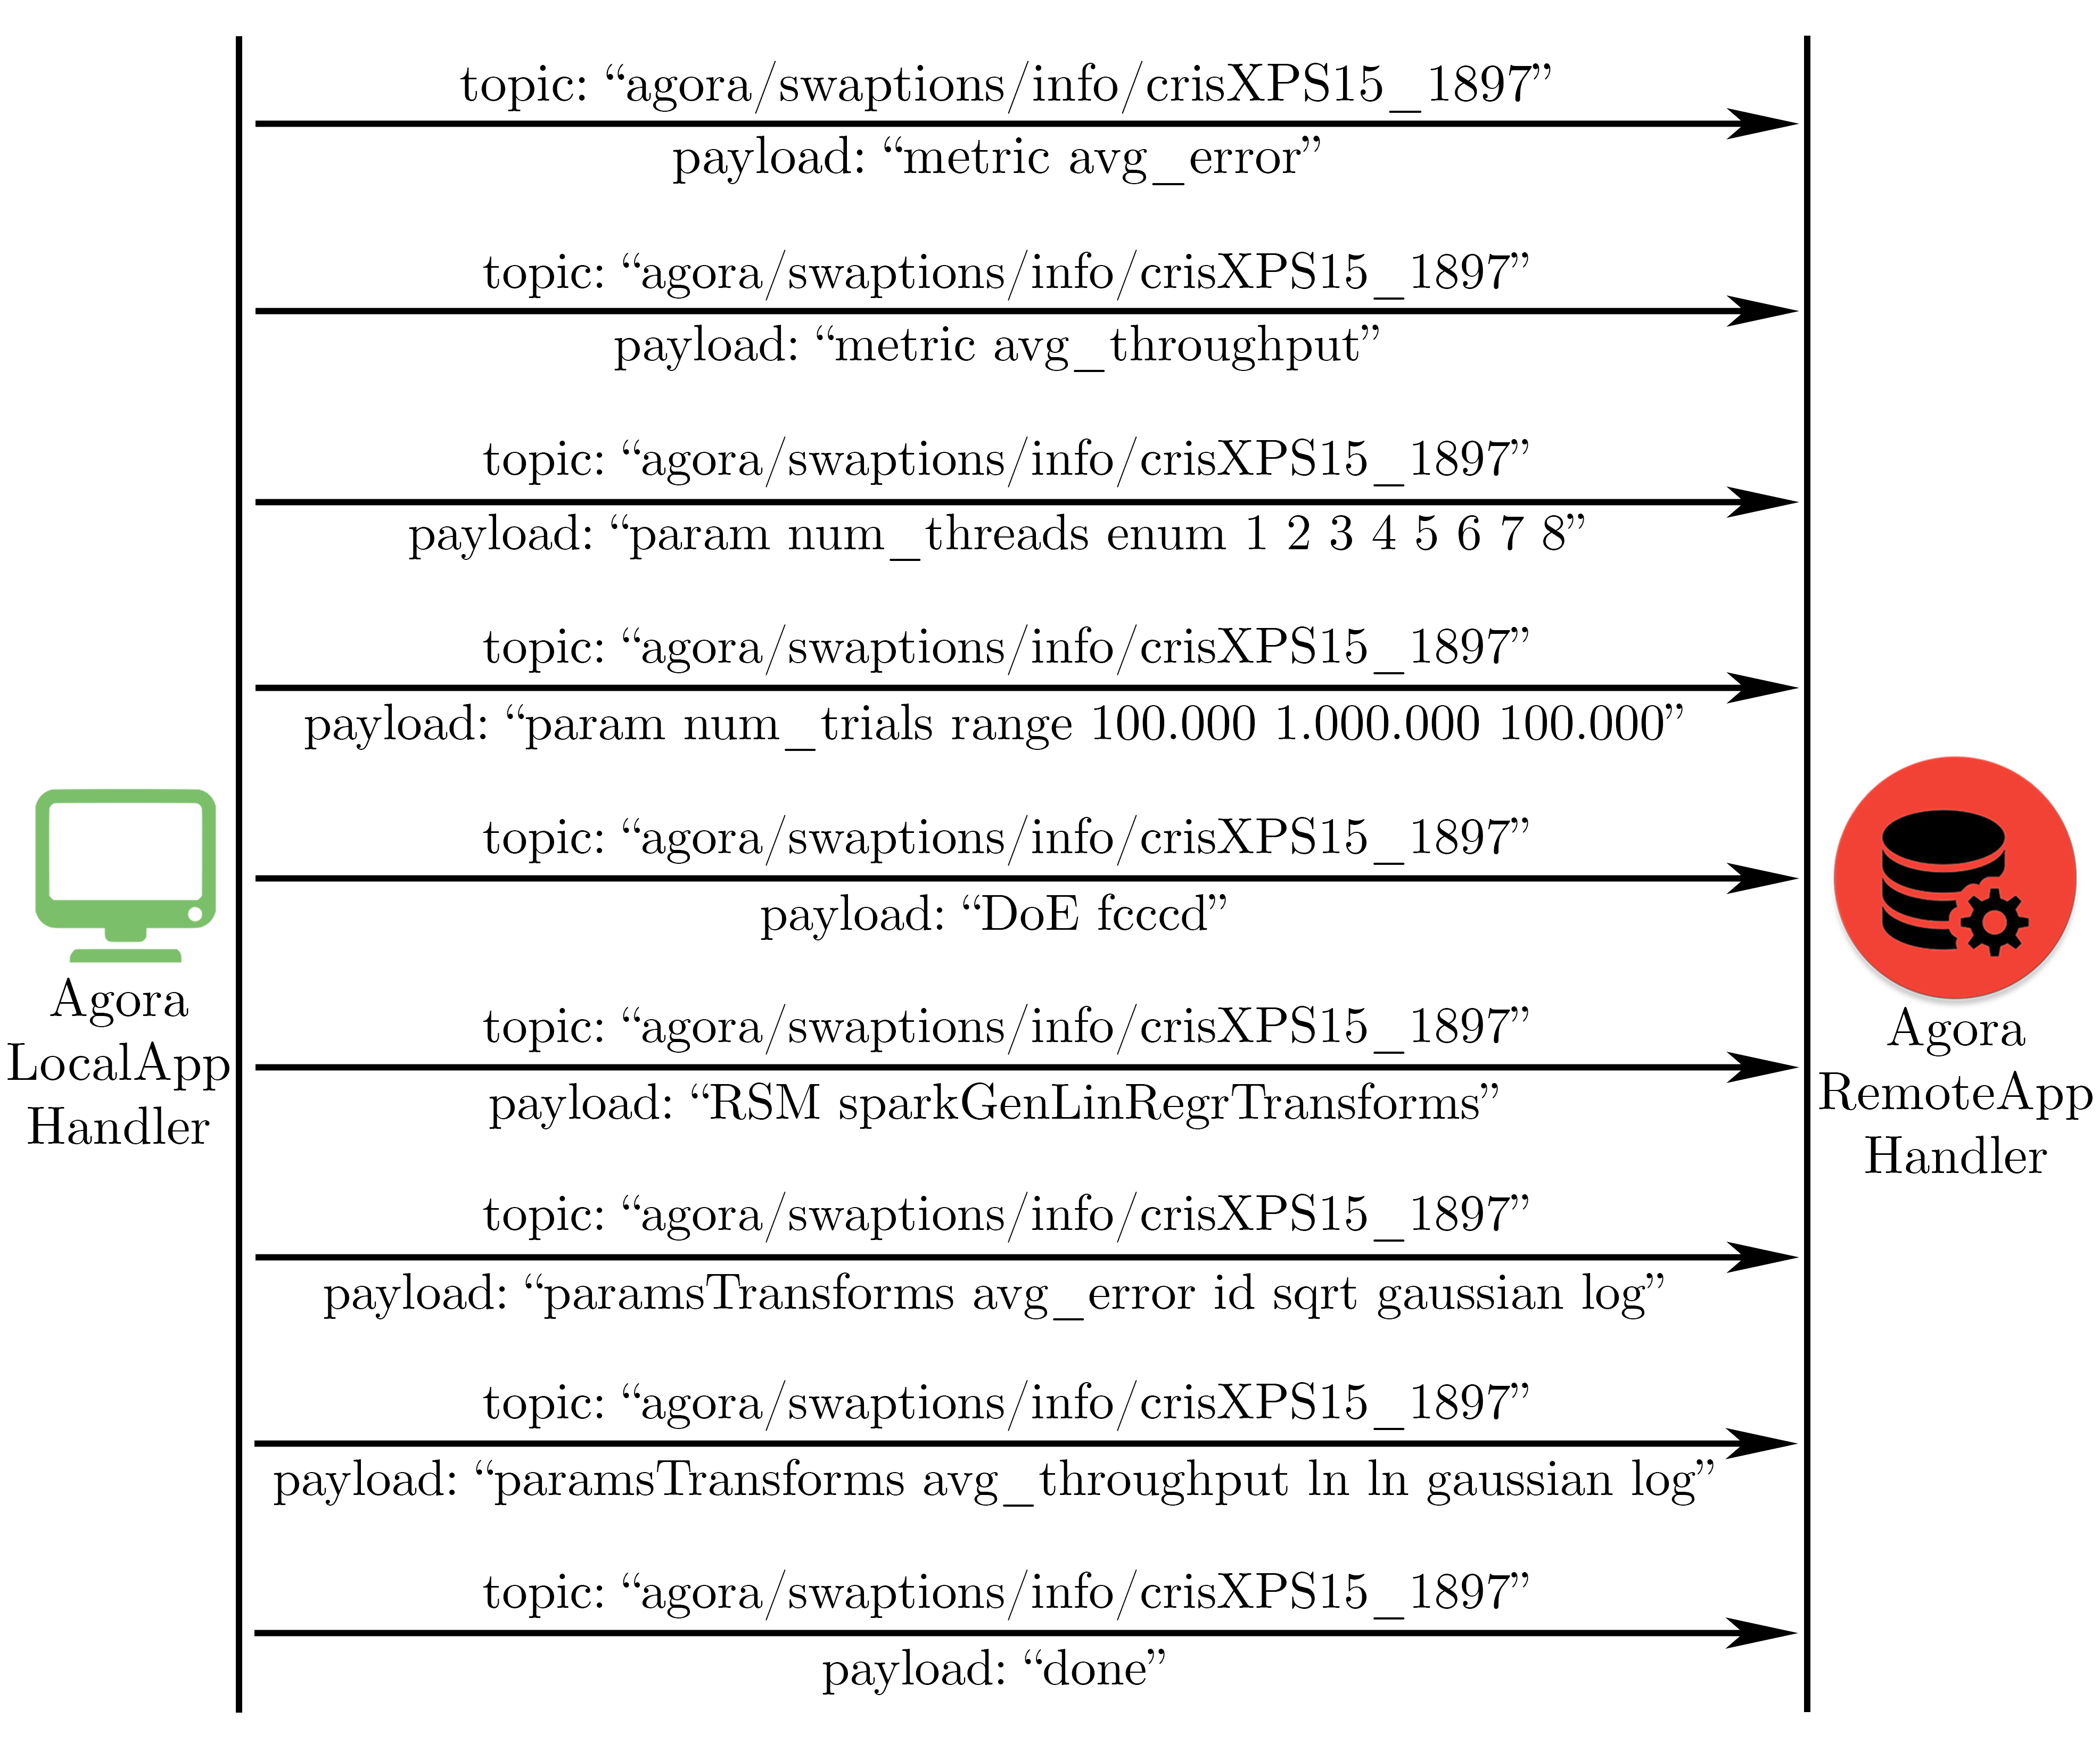
\includegraphics[width = \textwidth]{info_send}
    \caption{Application information dispatch by \textit{AgoràLocalAppHandler} module example}
    \label{fig:info_send}
    
\end{figure}

Taking figure \ref{fig:info_send} as reference, the AgoràRemoteAppHandler pulls out, from topic, \textit{crisXPS15\_1897} and it saves this identifier as the AgoràLocalAppHandler that is sending program information; as we can see, \textit{Swaptions} application focuses on two metrics, $avg\_error$ and $avg\_throughput$; it has two parameters, $num\_threads$ and $num\_trials$; the former is sent with the complete list of values, while the latter is sent with the keyword \textit{range}, specifying its minimum value ($100.000$), its maximum one ($1.000.000$) and the step ($100.000$): the Agorà\-Remote\-App\-Handler computes all values, that are therefore $100.000$, $200.000$, $300.000$, ..., $1.000.000$; the Design of Experiments that has to be used is the Face Centered DoE with one Center Point and the RSM technique is the 1st version of the Apache Spark\textsuperscript{TM} Generalized Linear Regression; parameter transformations are also specified so, e.g. for metric $avg\_error$, the first parameter ($num\_threads$) will not be transformed, while the second parameter ($num\_trials$) has to be transformed with the square root function, applying \textit{gaussian} as family distribution and \textit{log} as link function; it can be noticed that there is no information about the number of Operating Point repetitions to collect during DSE phase: in this case, default value is used (1 repetition for each OP); finally, there is no payload with keyword \textit{numFeats} either: \textit{Swaptions} does not have features.

The AgoràRemoteAppHandler module is now ready to compute Design of Experiments configurations; after that, it can start distributing them to nodes, driving the subsequent Design Space Exploration phase.





\subsection{Operating Point dispatch by AgoràLocalAppHandler module}\label{opSend}

During DSE, AgoràLocalAppHandler modules store configurations that receive from AgoràRemoteAppHandler (see \ref{dse_conf}); every time a configuration is sent, if the one in use differs from the new one, AgoràLocalAppHandler communicates to mARGOt autotuner new parameter values, therefore next program computation is executed with new parameter values.

When execution is finished, the AgoràLocalAppHandler module arranges the obtained Operating Point, composed by the set of parameter values and the observed metrics of interest; it publishes on topic "agora/\textit{[appName]}/OPs" a message in the form "\textit{[configuration]}:\textit{[metric values]}", in which both value lists have to follow lexicographic order with respect to parameter and metric name; if there are application features, payload is in the form "\textit{[configuration]}:\textit{[ob\-served feature values]}:\textit{[metric values]}":

\begin{figure}[H]

    \centering
    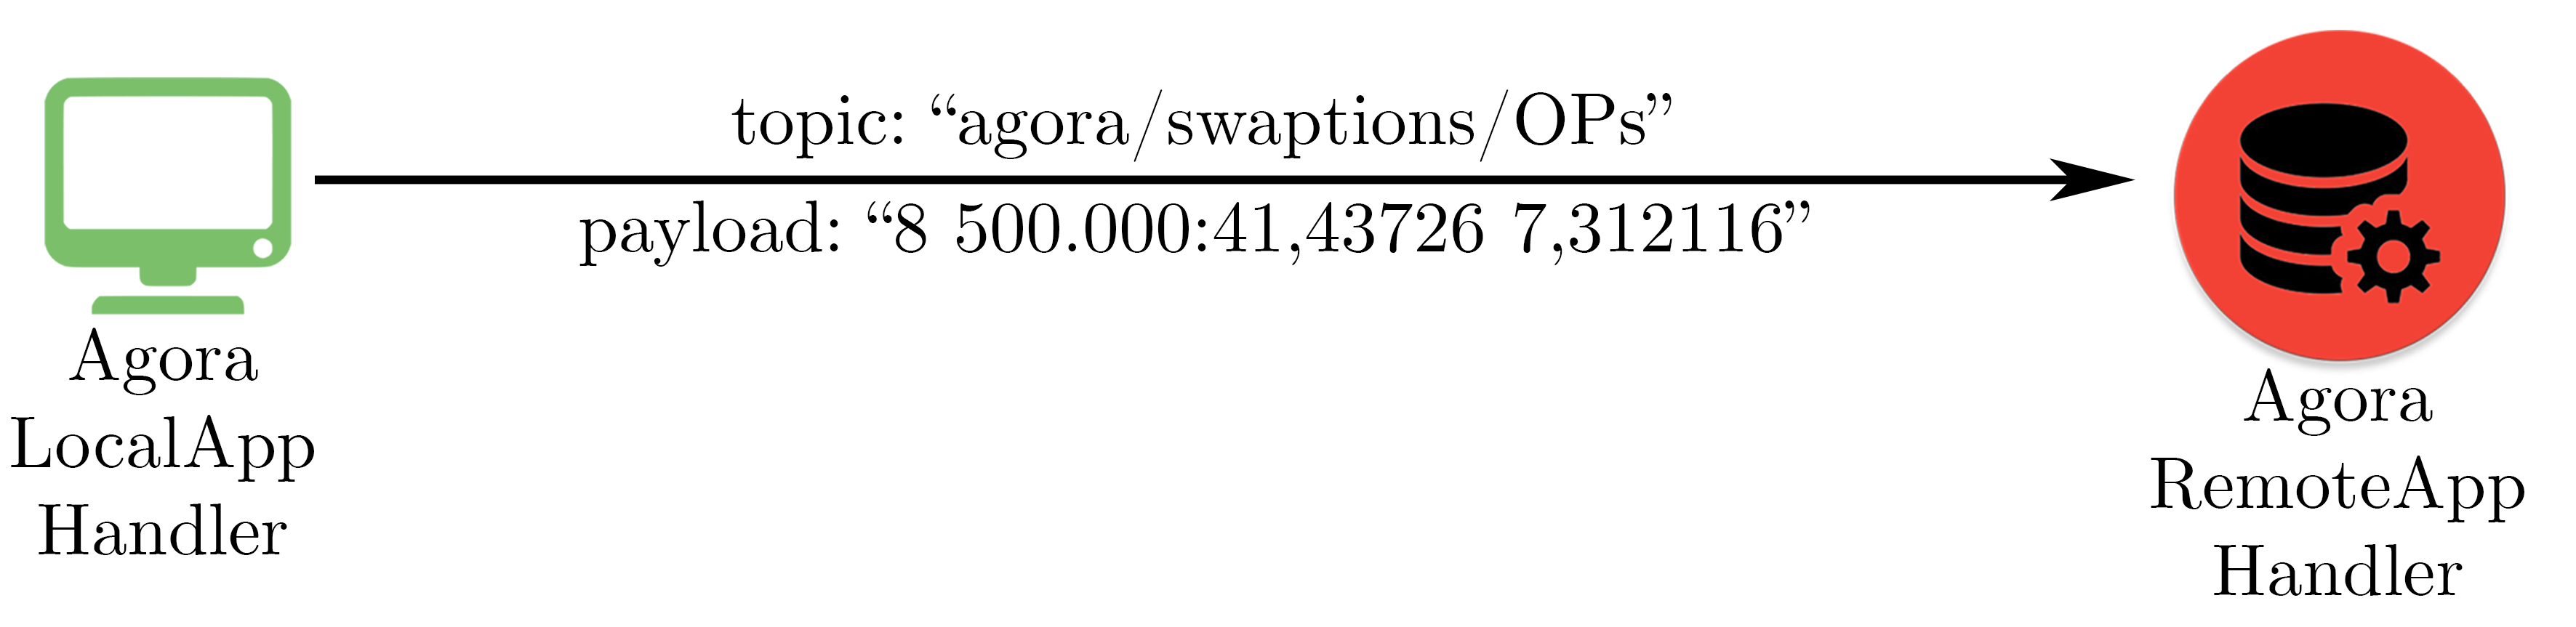
\includegraphics[width = \textwidth]{op}
    \caption{Operating Point dispatch by \textit{AgoràLocalAppHandler} module example}
    \label{fig:op}
    
\end{figure}

In the example above, \textit{Swaptions} has been just executed with\linebreak $num\_threads = 8$ and $num\_trials = 500.000$; monitored metric values are $avg\_error = 41,43726$ and $avg\_throughput = 7,312116$.

When AgoràRemoteAppHandler receives an Operating Point, it decrements the corresponding number of needed OP repetitions: if the updated value is equal to zero, it means that there is no need of other related OPs, so the corresponding configuration is moved from the set of available ones to the set of accomplished ones.

Model prediction just starts when last needed Operating Point repetition related to last available configuration is received from a node.





\subsection{AgoràLocalAppHandler module disconnection}\label{client_disc}

If an AgoràLocalAppHandler module disconnects for some reason, related Agorà\-Remote\-App\-Handler receives a message on topic "agora\slash{}\textit{[appName]}\slash{}disconnection" with payload "\textit{[hostname]\_[PID]}", relative to disconnected AgoràLocalAppHandler; the AgoràRemote\-App\-Handler module removes node identifier from the list of machines it is managing:

\begin{figure}[H]

    \centering
    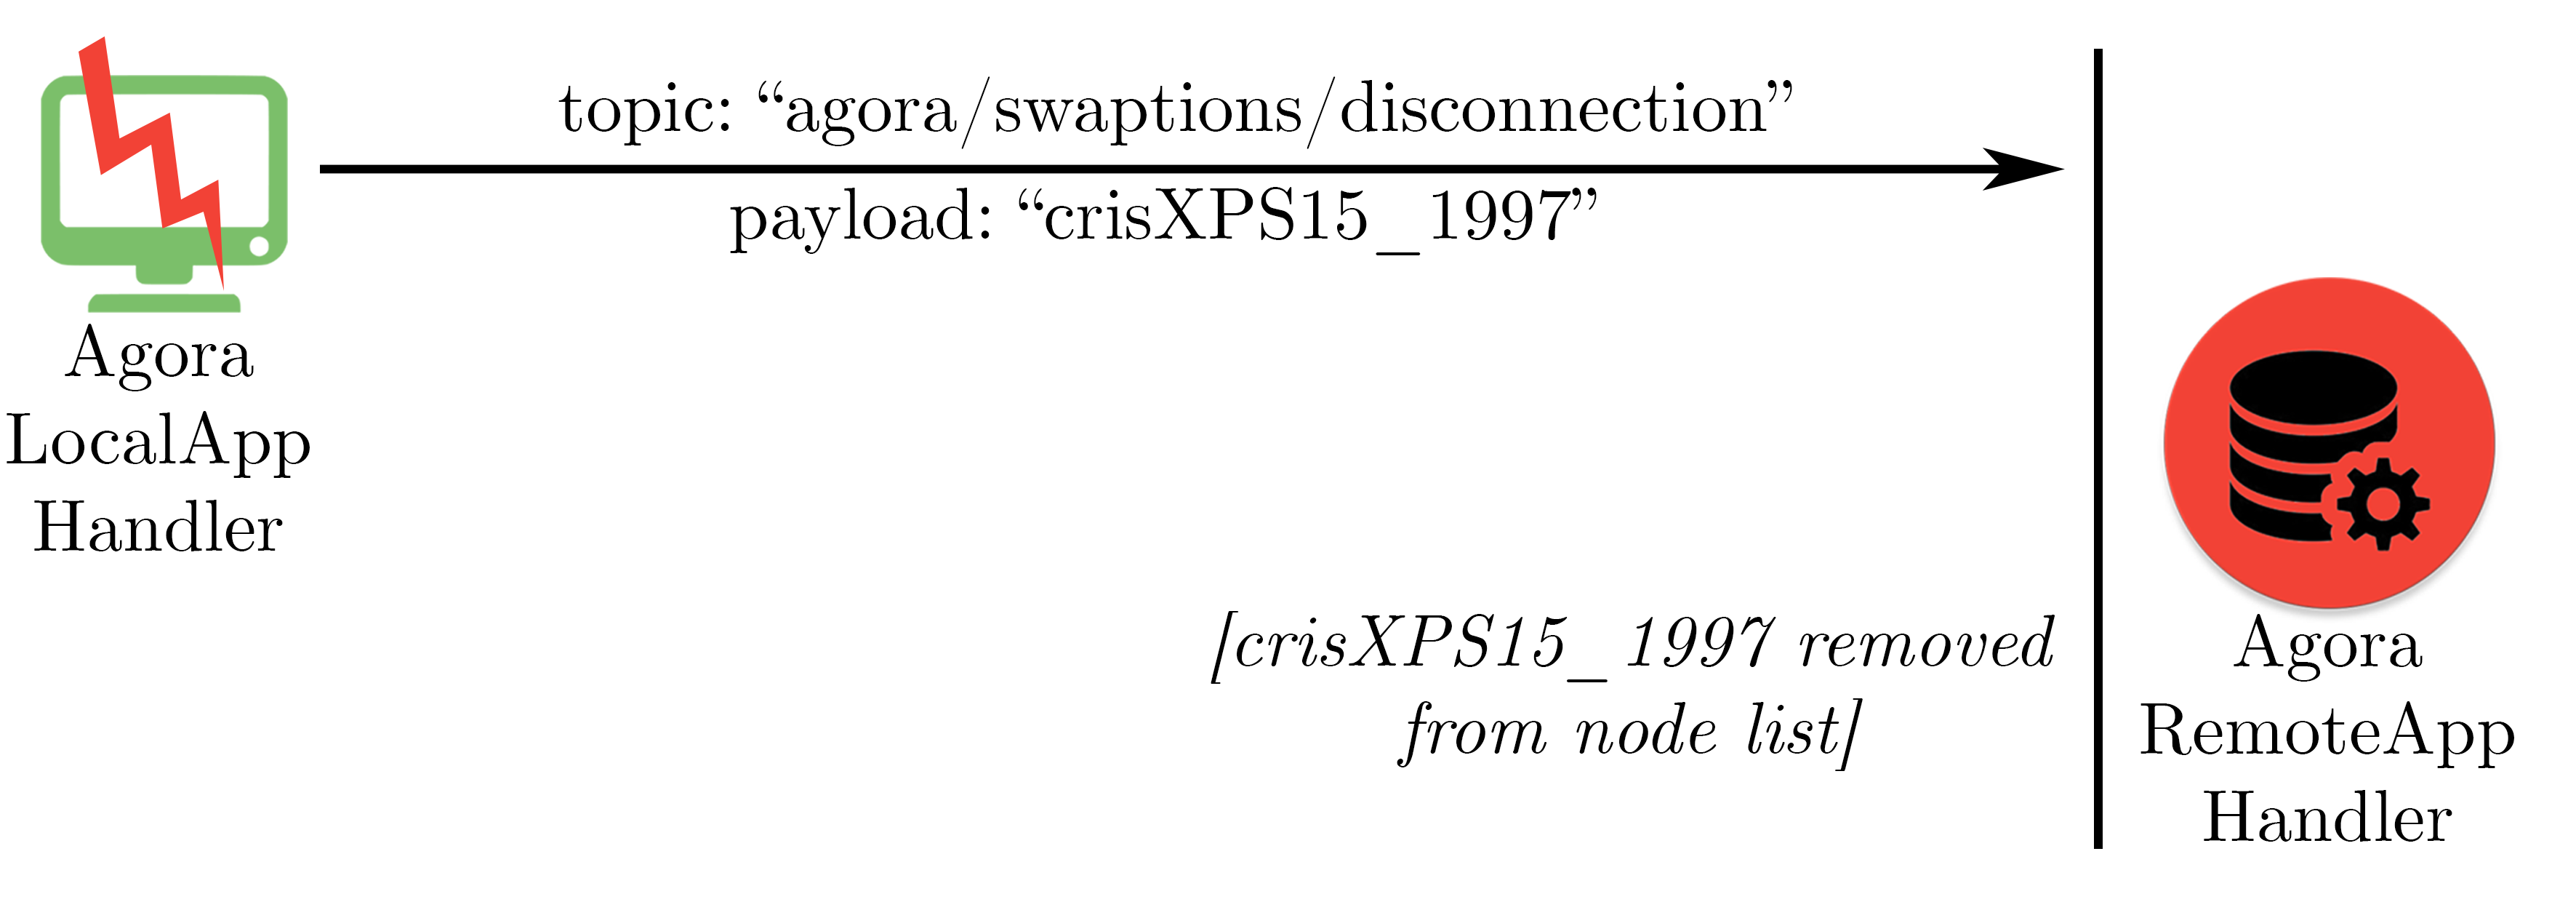
\includegraphics[width = \textwidth]{client_disc}
    \caption{AgoràLocalAppHandler module disconnection example}
    
\end{figure}

Particular attention has to be taken if the disconnected AgoràLocalAppHandler module is the one that, at the beginning, is sending application information (see \ref{client_info}): in this case, AgoràRemoteAppHandler has to remove disconnected machine, it has to reset partial data (received up to that moment) and it asks again all available application information to remaining connected AgoràLocalAppHandler modules:

\begin{figure}[H]

    \centering
    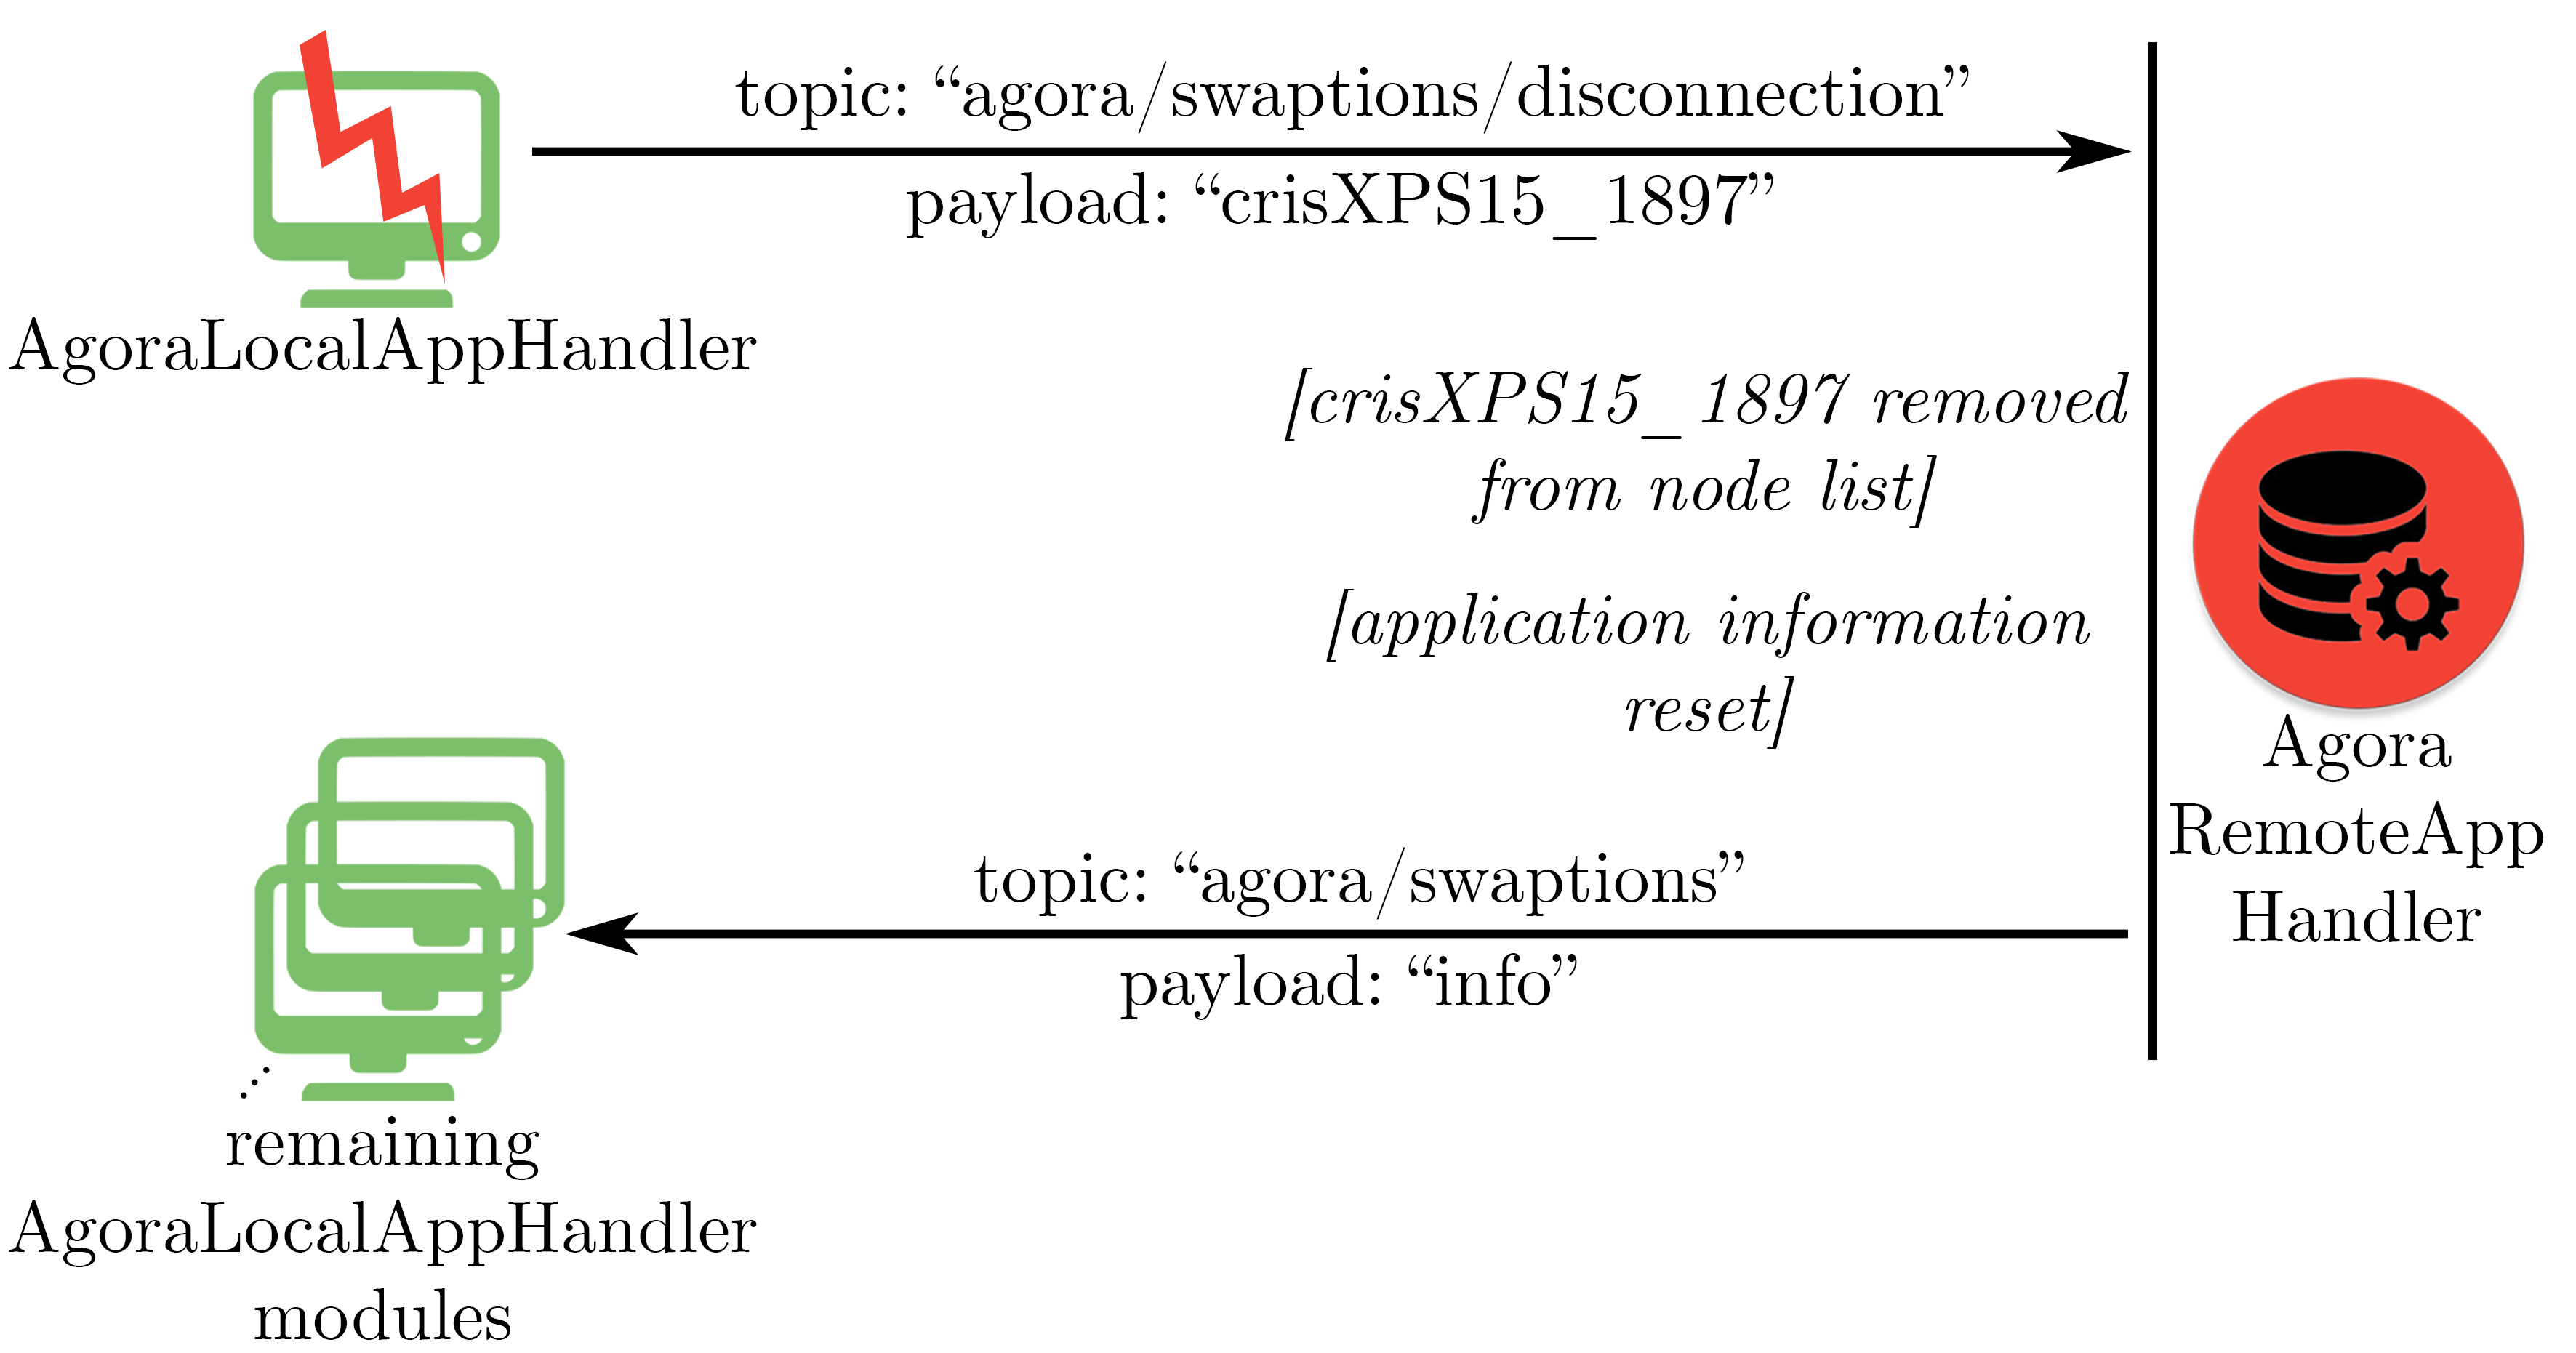
\includegraphics[width = \textwidth]{infoclient_disc}
    \caption{Disconnection of \textit{AgoràLocalAppHandler} module that was sending application information example}
    
\end{figure}





\subsection{AgoràRemoteAppHandler module disconnection}\label{handler_disc}

If the AgoràRemoteAppHandler module disconnects, related AgoràLocalAppHandler modules receive a message on topic "agora\slash{}\textit{[appName]}" with payload "disconnection":

\begin{figure}[H]

    \centering
    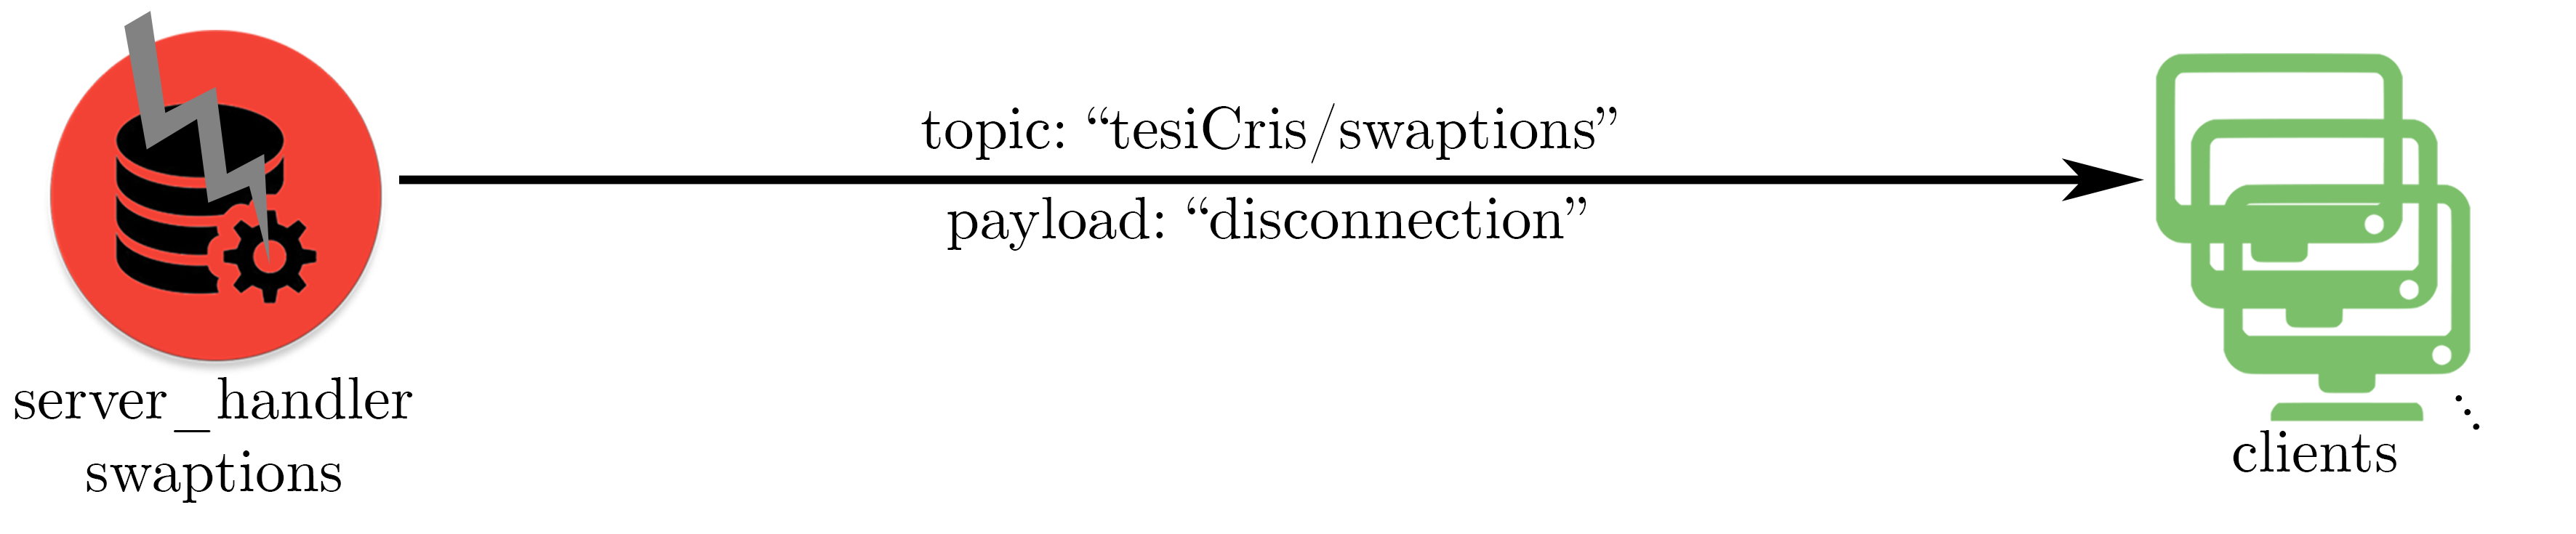
\includegraphics[width = \textwidth]{server_disc}
    \caption{AgoràRemoteAppHandler module disconnection example}
    
\end{figure}

Each AgoràLocalAppHandler reacts to this event according to its internal state, that can be:

\begin{enumerate}

    \item \textit{defaultStatus};
    
    \item \textit{DSE};
    
    \item \textit{DoEModel};
    
    \item \textit{autotuning}.

\end{enumerate}


\subsubsection{AgoràLocalAppHandler internal state equal to \textit{defaultStatus}}

When a node starts running a program, the autotuner sets up application parameter values with a predetermined default configuration; if any Design Space Exploration phase has not been started yet, AgoràRemoteAppHandler disconnection does not affect application behavior.


\subsubsection{AgoràLocalAppHandler internal state equal to \textit{DSE}}

The AgoràRemoteAppHandler module is driving Design Space Exploration phase, sending configurations to AgoràLocalAppHandler modules; in this case, default configuration is restored and the application is executed with corresponding parameter values:

\begin{figure}[H]

    \centering
    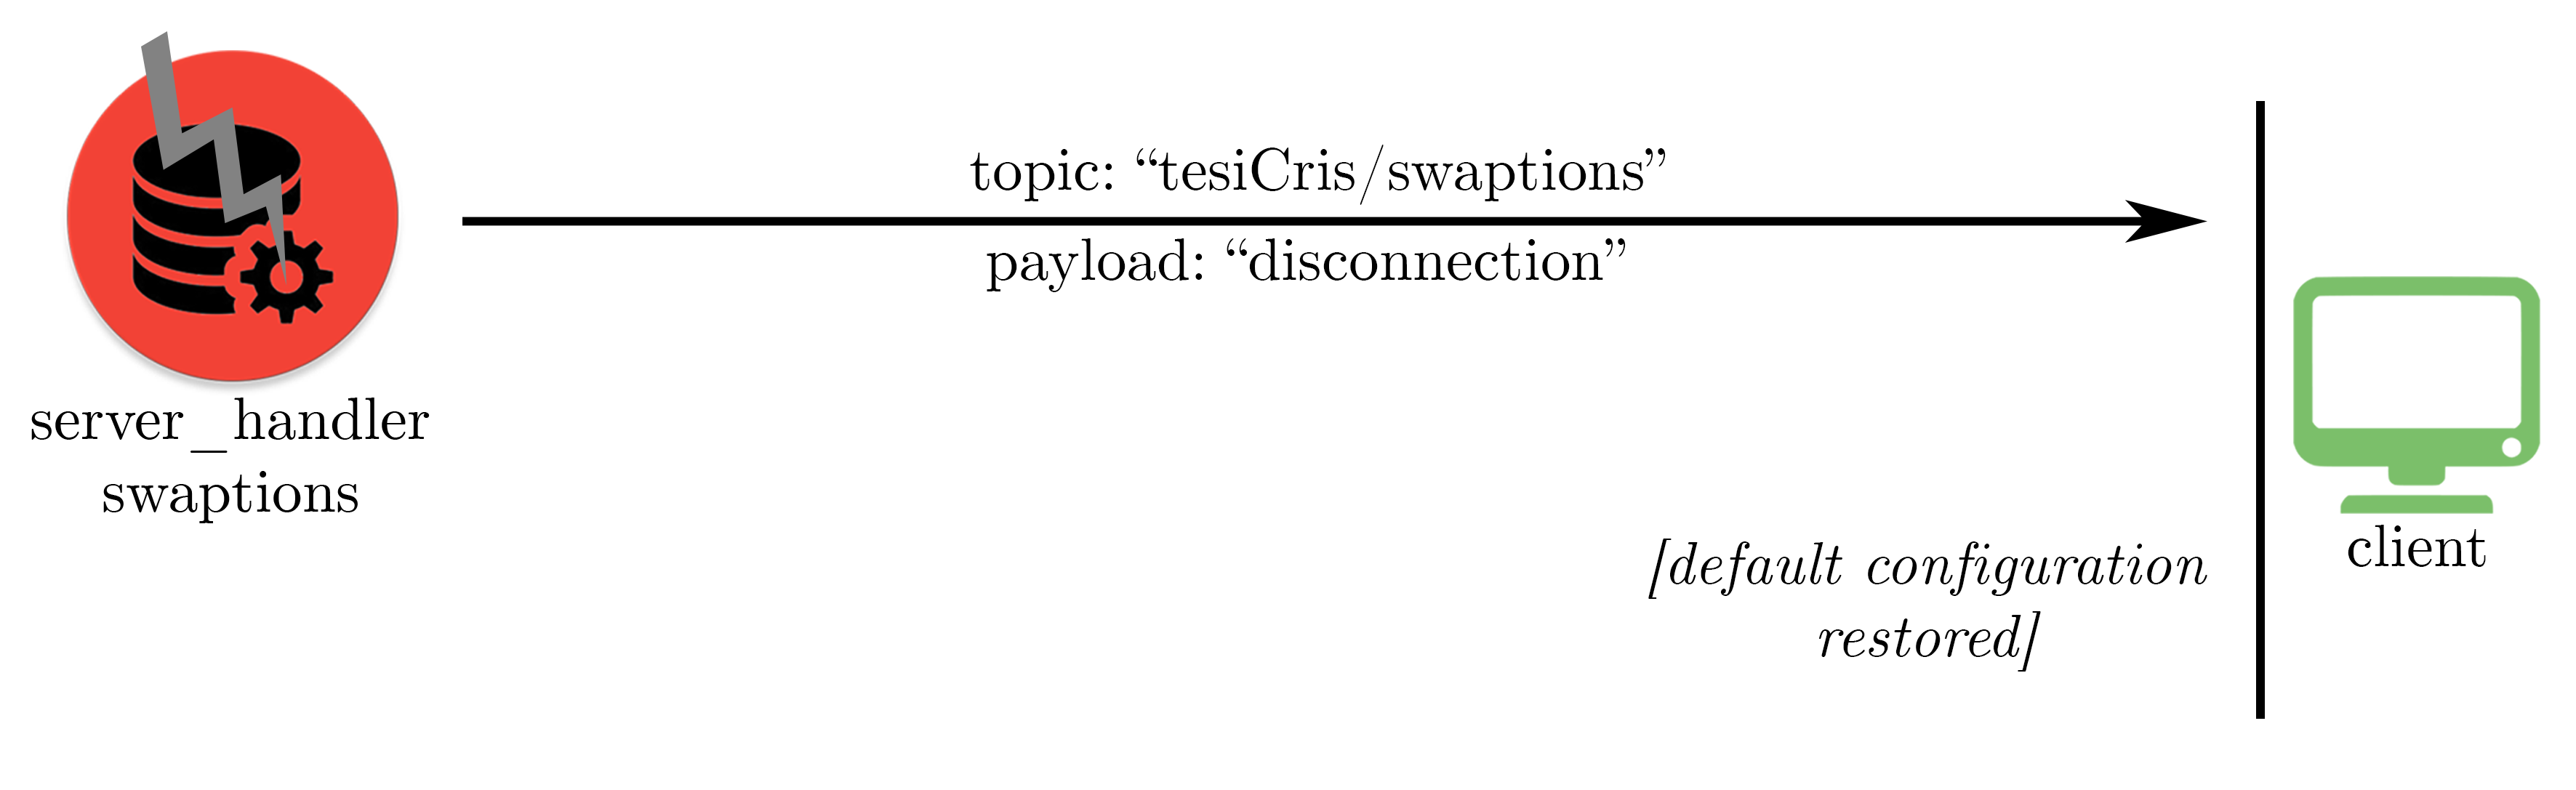
\includegraphics[width = \textwidth]{DSEinternal}
    \caption{AgoràRemoteAppHandler module disconnection with AgoràLocalAppHandler internal state equal to \textit{DSE} example}
    
\end{figure}


\subsubsection{AgoràLocalAppHandler internal state equal to \textit{DoEModel}}

AgoràLocalAppHandler has received a partial OP list, related to Design of Experiments configurations (see \ref{DoEModelSend}); in this case, available OP list is not deleted, therefore the autotuner continues to work with this information.


\subsubsection{AgoràLocalAppHandler internal state equal to \textit{autotuning}}

The AgoràLocalAppHandler module has already received predicted complete OP list from AgoràRemoteAppHandler, therefore nothing changes.





\section{AgoràLocalAppHandler module integration}

\begin{figure}[H]

    \centering
    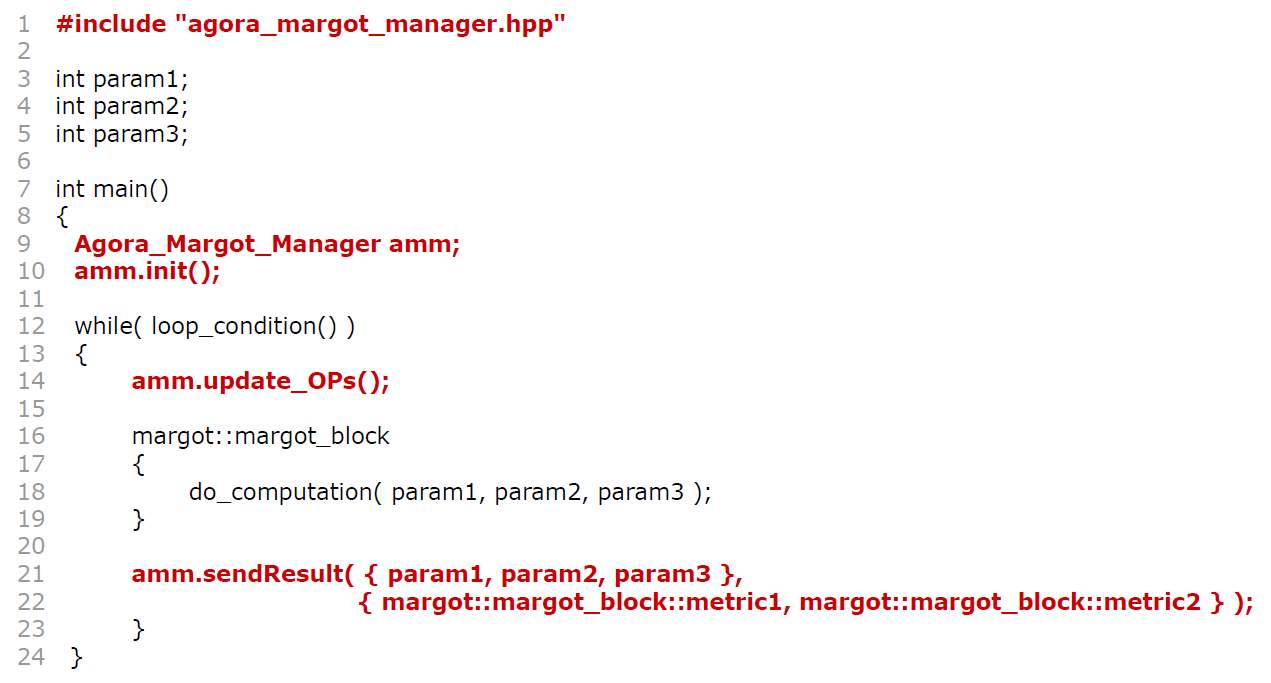
\includegraphics[width = \textwidth]{tesiCris_client_integration}
    \caption{Sketch application with \textit{AgoràLocalAppHandler} module plus mARGOt autotuner integration}
    \label{fig::sketchApp}
    
\end{figure}

Figure \ref{fig::sketchApp} shows a sketch application that, until \textit{loop\_condition()} is verified (line 12), is executed; computation depends on three parameters ($param1, param2, param3$) that are set up by mARGOt autotuner at the beginning of every cycle (line 16), while two metrics of interest ($metric1, metric2$) are monitored (for mARGOt details, see related scientific publication \cite{gadioli2015application}).

Integration code required to use Agorà framework with mARGOt autotuner is written in bold red; main steps during program execution are three:

\begin{enumerate}

    \item AgoràLocalAppHandler module and mARGOt autotuner instantiation and initialization (lines 9-10): the AgoràLocalAppHandler module saves all application information and sets up mARGOt autotuner with a default Operating Point; if nothing happens, the application is executed with this configuration;
    
    \item Application knowledge update (line 14): the AgoràLocalAppHandler module updates, from time to time, its internal knowledge about application configurations that are sent by the AgoràRemoteAppHandler module; before mARGOt autotuner sets up application parameters (line 16), AgoràLocalAppHandler checks mARGOt knowledge with respect to its internal one: if they are different, mARGOt Operating Points are updated. In this way, for instance, if the AgoràLocalAppHandler module receives a new configuration during Design Space Exploration phase (see \ref{dse_conf}), mARGOt knowledge is set up with this data, so the application is forced to be executed with the corresponding parameter values; if, for instance, application complete model is received (see \ref{modelSend}), mARGOt internal knowledge is set up with all this information, so the autotuner can choose the best Operating Point that fulfills application current goals and requirements;
    
    \item Operating Point dispatch (line 21-22): after each computation has done, parameter values just used with the corresponding monitored metrics of interest are published on a predetermined MQTT topic, so the related AgoràRemoteAppHandler module can receive this information (see \ref{opSend}).
    
\end{enumerate}
